%convert -coalesce launch.gif launch_%d.png
\documentclass{beamer}

\newcommand{\VEV}[1]{\langle#1\rangle}
\newcommand{\sst}{\left(1-\frac{2M}{r}\right)}
\newcommand{\sh}{\mathrm{shell}}
\newcommand{\be}{\begin{equation}}
\newcommand{\ee}{\end{equation}}
\newcommand{\bue}{\begin{equation}}
\newcommand{\eue}{\end{equation}}
\newcommand{\bc}{\begin{center}}
\newcommand{\ec}{\end{center}}
\newcommand{\bea}[1]{\begin{eqnarray}\label{#1}}
\newcommand{\eea}{\end{eqnarray}}
\newcommand{\bua}{\begin{eqnarray*}}
\newcommand{\eua}{\end{eqnarray*}}
\newcommand{\dd}[2]{{{d#1}\over{d#2}}}
\newcommand{\ddt}[1]{\dd{#1}{t}}
\newcommand{\dddt}[1]{\dd{^2#1}{t^2}}
\newcommand{\aver}[1]{\langle{#1}\rangle}
\newcommand{\atom}[3]{\ifmmode^{#1}_{#2}{\rm{#3}}\else{$^{#1}_{#2}${#3}}\fi}
\newcommand{\electron}{\atom{~0}{-1}{e}}
\newcommand{\positron}{\atom{0}{0}{\bar{e}}}
\newcommand{\neutrino}{\atom{0}{0}{\nu_e}}
\newcommand{\photon}{\atom{0}{0}{\gamma}}
\newcommand{\antineutrino}{\atom{0}{0}{\bar{\nu}}}
\newcommand{\neutron}{\atom{1}{0}{n}}
\newcommand{\proton}{\atom{1}{1}{p}}
\newcommand{\hydrogen}{\atom{1}{1}{H}}
\newcommand{\deuterium}{\atom{2}{1}{H}}
\newcommand{\tritium}{\atom{3}{1}{H}}
\newcommand{\helium}{\atom{4}{2}{He}}
\newcommand{\hethree}{\atom{3}{2}{He}}

\renewcommand{\ss}{Schwarz\-schild }

\def\densu{kg/m$^3$} 
\def\rsol{R$_{\odot}$} 
\def\msol{M$_{\odot}$} 

\newcommand{\htmlcom}[1]{}


\usetheme{Boadilla}
%\usepackage{multimedia}
%\usepackage{animate}
\usepackage{hyperref}
\usepackage{tikz}
\usepackage{cancel}
\usepackage{tikzsymbols}
\usepackage{ifthen}

%%%%mathcircled
\makeatletter
\newcommand\mathcircled[1]{%`
  \mathpalette\@mathcircled{#1}%
}
\newcommand\@mathcircled[2]{%
  \tikz[baseline=(math.base)] \node[draw,circle,red, thick, inner sep=2pt] (math) {$\m@th#1#2$};%
}
\makeatother
%%%%

%gets rid of bottom navigation bars
\setbeamertemplate{footline}[frame number]{} %begin

%gets rid of bottom navigation symbols
\setbeamertemplate{navigation symbols}{}

%gets rid of footer
%will override 'frame number' instruction above  %begin
%comment out to revert to previous/default definitions
\setbeamertemplate{footline}{}

\definecolor{darkscarlet}{rgb}{0.34, 0.01, 0.1}
\definecolor{gold(metallic)}{rgb}{0.83, 0.69, 0.22}
\definecolor{green(ryb)}{rgb}{0.4, 0.69, 0.2}
\definecolor{darkorange}{rgb}{1.0, 0.55, 0.0}
\definecolor{amber}{rgb}{1.0, 0.75, 0.0}
\definecolor{bronze}{rgb}{0.8, 0.5, 0.2}
\definecolor{cadet}{rgb}{0.33, 0.41, 0.47}
\definecolor{silver}{rgb}{0.75, 0.75, 0.75}
\definecolor{turquoise}{rgb}{0.19, 0.84, 0.78}
\definecolor{uclagold}{rgb}{1.0, 0.7, 0.0}
\definecolor{urobilin}{rgb}{0.88, 0.68, 0.13}
\definecolor{vegasgold}{rgb}{0.77, 0.7, 0.35}
\definecolor{vanilla}{rgb}{0.95, 0.9, 0.67}
\definecolor{straw}{rgb}{0.89, 0.85, 0.44}
\definecolor{sunset}{rgb}{0.98, 0.84, 0.65}
\definecolor{brown(traditional)}{rgb}{0.59, 0.29, 0.0}
\definecolor{apricot}{rgb}{0.98, 0.81, 0.69}
\definecolor{darkblue}{rgb}{0,0,0.54}

\hypersetup{
    colorlinks=true,
    linkcolor=yellow,
    filecolor=magenta,
    urlcolor=blue,
}

\let\hrefori\href
\renewcommand{\href}[2]{{\setlength{\fboxsep}{1pt}\colorbox{sunset}{\hrefori{#1}{#2}}}}


%title
\setbeamercolor{block title alerted}{fg=white,bg=cyan}
%body
\setbeamercolor{block body alerted}{fg=black!90,bg=yellow!60}

%title
\setbeamercolor{block title}{fg=black,bg=turquoise}
%body
\setbeamercolor{block body}{fg=yellow,bg=bronze}




\newcommand{\pagebutton}[1]{\setbeamertemplate{button}{\tikz\node[inner xsep = 5pt, draw = structure!90, fill = green(ryb), rounded corners = 8pt]{\color{amber}\Large\insertbuttontext};}\beamerbutton{#1}}

\newcommand{\choicebutton}[1]{\setbeamertemplate{button}{\tikz\node[inner xsep = 8pt, draw = structure!90, fill = vegasgold, rounded corners = 5pt]{\color{vanilla}\Large\insertbuttontext};}\beamerbutton{#1}}

\newcommand{\pagenobutton}[1]{\setbeamertemplate{button}{\tikz\node[inner xsep = 8pt, draw = structure!90, fill = apricot, rounded corners = 5pt]{\color{brown(traditional)}\Large\insertbuttontext};}\beamerbutton{#1}}

\newcommand{\headlinebutton}[1]{\setbeamertemplate{button}{\tikz\node[inner xsep = 8pt, draw = structure!90, fill = blue, rounded corners = 5pt]{\color{yellow}\Large\insertbuttontext};}\beamerbutton{#1}}

\newcommand{\forumbutton}{\href{https://astro-discourse.utenforuio.no/c/ast2000/sporsmal-til-ukeoppgavene-i-del-2a-2d/11}{\setbeamertemplate{button}{\tikz\node[inner xsep = 8pt, draw = structure!90, fill = darkblue, rounded corners = 5pt]{\color{yellow}\Large\insertbuttontext};}\beamerbutton{\textcolor{red}{\small FORUM}}}}

\newcommand{\curpage}{\pagenobutton{\small side \thepageno\  av \thenopages}}
\newcommand{\nextpage}{\refstepcounter{pageno}\pagenobutton{\small side \thepageno\  av \thenopages}}
\newcommand{\dnextpage}{\refstepcounter{pageno}\refstepcounter{pageno}\pagenobutton{\small side \thepageno\  av \thenopages}}

\newcommand{\lastpagebutton}[1]{\hyperlink{#1}{\pagebutton{\small Forrige side}}\href{https://nettskjema.no/a/170171}{\Changey[1][yellow]{2} \Changey[1][yellow]{-2}}\nextpage\headlinebutton{\headline}\forumbutton}
\newcommand{\clastpagebutton}[1]{\hyperlink{#1}{\pagebutton{\small Forrige side}}\href{https://nettskjema.no/a/170171}{\Changey[1][yellow]{2} \Changey[1][yellow]{-2}}\curpage\headlinebutton{\headline}\forumbutton}
\newcommand{\dlastpagebutton}[1]{\hyperlink{#1}{\pagebutton{\small Forrige side}}\href{https://nettskjema.no/a/170171}{\Changey[1][yellow]{2} \Changey[1][yellow]{-2}}\dnextpage\headlinebutton{\headline}\forumbutton}

\newcommand{\lastpagebuttonx}[1]{\hyperlink{#1}{\pagebutton{\small Forrige side}}\href{https://nettskjema.no/a/170171}{\Changey[1][yellow]{2} \Changey[1][yellow]{-2}}\nextpage\\}
\newcommand{\clastpagebuttonx}[1]{\hyperlink{#1}{\pagebutton{\small Forrige side}}\href{https://nettskjema.no/a/170171}{\Changey[1][yellow]{2} \Changey[1][yellow]{-2}}\curpage\\}
\newcommand{\dlastpagebuttonx}[1]{\hyperlink{#1}{\pagebutton{\small Forrige side}}\href{https://nettskjema.no/a/170171}{\Changey[1][yellow]{2} \Changey[1][yellow]{-2}}\dnextpage\\}

\newcommand{\lastpagebuttoncr}[1]{\hyperlink{#1}{\pagebutton{\small Forrige side}}\href{https://nettskjema.no/a/170171}{\Changey[1][yellow]{2} \Changey[1][yellow]{-2}}\nextpage\\\headlinebutton{\headline}\forumbutton\\}
\newcommand{\clastpagebuttoncr}[1]{\hyperlink{#1}{\pagebutton{\small Forrige side}}\href{https://nettskjema.no/a/170171}{\Changey[1][yellow]{2} \Changey[1][yellow]{-2}}\curpage\\\headlinebutton{\headline}\forumbutton\\}
\newcommand{\dlastpagebuttoncr}[1]{\hyperlink{#1}{\pagebutton{\small Forrige side}}\href{https://nettskjema.no/a/170171}{\Changey[1][yellow]{2} \Changey[1][yellow]{-2}}\dnextpage\\\headlinebutton{\headline}\forumbutton\\}

\newcommand{\nytemaside}[1]{
\centerline{\Huge\textcolor{yellow}{Nytt tema:}}\\
\vspace*{1cm}
\centerline{\Large\bf\textcolor{yellow}{\headline}}
\vspace*{2cm}
\ifthenelse{\equal{#1}{0}}{\centerline{\textcolor{yellow}{Siste tema i denne forelesningen!}}}{\centerline{\textcolor{yellow}{\footnotesize Dette temaet fortsetter frem til side \ref{#1} av \thenopages.}}}
\vspace*{0.5cm}
}


\newcommand{\fullframe}[6]{
\begin{frame}
\label{#1}
\addtocounter{pageno}{#4}
\lastpagebutton{#2}{\bf #6}\\
#5
\hyperlink{#3}{\pagebutton{Neste side}}
\end{frame}
}



\newcommand{\fullframetwo}[7]{
\begin{frame}
\label{#1}
\addtocounter{pageno}{#4}
\lastpagebutton{#2}{\bf #7}\\
\begin{columns}
\column{0.5\textwidth}
#5
\column{0.5\textwidth}
#6
\hyperlink{#3}{\pagebutton{Neste side}}
\end{columns}
\end{frame}
}

\newcommand{\fullframetwonotxt}[7]{
\begin{frame}
\label{#1}
\addtocounter{pageno}{#4}
\lastpagebutton{#2}{\bf #7}\\
\begin{columns}
\column{0.5\textwidth}
#5
\column{0.5\textwidth}
#6
\end{columns}
\end{frame}
}



\newcommand{\fullframetxt}[7]{
\begin{frame}
\label{#1}
\addtocounter{pageno}{#4}
\lastpagebutton{#2}{\bf #7}\\
#6
\hyperlink{#3}{\pagebutton{#5}}
\end{frame}
}

\newcommand{\fullframenotxt}[6]{
\begin{frame}
\label{#1}
\addtocounter{pageno}{#4}
\lastpagebutton{#2}{\bf #6}\\
#5
\end{frame}
}

\newcommand{\choiceframe}[5]{
\begin{frame}
\label{#1}
\addtocounter{pageno}{#3}
\lastpagebutton{#2}{\bf #5}\\
#4
\end{frame}
}

\newcommand{\colfullframe}[7]{
{
\setbeamercolor{background canvas}{bg=#5}
\begin{frame}
\label{#1}
\addtocounter{pageno}{#4}
\lastpagebutton{#2}{\bf #7}\\
#6
\hyperlink{#3}{\pagebutton{Neste side}}
\end{frame}
}
}

\newcommand{\colfullframetwo}[8]{
{
\setbeamercolor{background canvas}{bg=#5}
\begin{frame}
\label{#1}
\addtocounter{pageno}{#4}
\lastpagebutton{#2}{\bf #8}\\
\begin{columns}
\column{0.5\textwidth}
#6
\column{0.5\textwidth}
#7
\hyperlink{#3}{\pagebutton{Neste side}}
\end{columns}
\end{frame}
}
}

\newcommand{\colfullframetxt}[8]{
{
\setbeamercolor{background canvas}{bg=#5}
\begin{frame}
\label{#1}
\addtocounter{pageno}{#4}
\lastpagebutton{#2}{\bf #8}\\
#7
\hyperlink{#3}{\pagebutton{#6}}
\end{frame}
}
}

\newcommand{\colchoiceframe}[6]{
{
\setbeamercolor{background canvas}{bg=#4}
\begin{frame}
\label{#1}
\addtocounter{pageno}{#3}
\lastpagebutton{#2}{\bf #6}\\
#5
\end{frame}
}
}


\newcommand{\pagequestion}[3]{
\hyperlink{#1}{\pagebutton{#2}}
\pause
%#3 normalt -1 for første spørsmål
\addtocounter{pageno}{#3}
\begin{itemize}[<+->]
\item[] \hypertarget<.>{#1}{}
\end{itemize}
\vspace{-0.5cm}
}

\newcommand{\samepagequestion}[4]{
\hyperlink{#1}{\pagebutton{#2}}\hyperlink{#1}{\pagebutton{#3}}
\pause
%#3 normalt -1 for første spørsmål
\addtocounter{pageno}{#4}
\begin{itemize}[<+->]
\item[] \hypertarget<.>{#1}{}
\end{itemize}
\vspace{-0.5cm}
}

\newcommand{\twopagequestion}[7]{
\hyperlink{#1}{\pagebutton{#3}}\hyperlink{#2}{\pagebutton{#4}}
\pause
%#3 normalt -1 for første spørsmål
\addtocounter{pageno}{#5}
\begin{itemize}[<+->]
\item[] \hypertarget<.>{#1}{}
\end{itemize}
\vspace{-0.5cm}
#7
\addtocounter{pageno}{#6}
\begin{itemize}[<+->]
\item[] \hypertarget<.>{#1}{}
\end{itemize}
\vspace{-0.5cm}
}

\newcounter{pageno}
\newcounter{nopages}
\setcounter{nopages}{42}

\newcommand{\headline}{\small Introduksjon}
\newcommand{\m}{\mathrm{m}}

\begin{document}

\begin{frame}
\label{front2}
\center{\Large \textcolor{darkscarlet}{\bf AST2000 Del 2A\\Interaktive forelesningsnotater: forelesning 2 av 2}}\\
\begin{block}{\center{\bf VIKTIG}}
\textcolor{yellow}{Dette er et alternativ til forelesningen i emnet.} \textcolor{blue}{Har du gått skikkelig gjennom disse interaktive forelesningsnotatene så trenger du ikke å lese \href{https://www.uio.no/studier/emner/matnat/astro/AST2000/h21/undervisningsmateriell/lecture_notes/part2a.pdf}{de fulle forelesningsnotatene} (med unntak av oppgavene bak)}. All informasjonen du trenger, får du her. Du kommer til å få mange grublespørsmål og diskusjonsoppgaver, det er meningen at disse skal gjøres i grupper av minst 2, maks 4 studenter. {\bf Det er defor sterkt anbefalt at dere sitter sammen i grupper når dere går gjennom disse interaktive forelesningsnotatene, du vil få betydelig mer utbytte av dem på den måten}. {\bf Hvis du har kommentarer ris/ros til disse forelesningsnotatene eller til emnet, trykk på \href{https://nettskjema.no/a/170171}{\Changey[1][yellow]{2} \Changey[1][yellow]{-2}}\ knappen som du finner på alle sider.}
\end{block}
%\setbeamercolor{button}{bg=black,fg=yellow}
\hyperlink{front3}{\pagebutton{Trykk denne knappen for å begynne}}
\end{frame}

\begin{frame}
\label{front3}
{\Large
\begin{itemize}
\item HUSK at du får mer ut av de interaktive forelesningsnotatene når du gjør de sammen med noen. Diskusjonene med andre er svært viktige.
\item Det er mange spørsmål/grubliser underveis, sett dere selv en tidsgrense, 1 minutt på de korte, maks 4-5 minutter på de lenger. Ha en alarm ved siden av, ellers kommer dere til å bruke alt for langt tid. Har dere ikke fått det til etter kort tid, gå videre, se svaret og lær!
\item Er du i det minste tvil om noe, så finnes det en \forumbutton knapp, trykk det og still spørsmål med en gang mens du enda husker spørsmålet!
\end{itemize}
}
\hyperlink{tableofcontents}{\pagebutton{Trykk denne knappen for å begynne}}
\end{frame}

\begin{frame}
\label{tableofcontents}
\hyperlink{front3}{\pagebutton{Forrige side}}\\
Hvis du allerede har begynt på denne forelesningen og vil hoppe rett inn til et annet kapittel, kan du trykke her:
\begin{itemize}
\item \hyperlink{blue_nytema1}{\headlinebutton{Repetisjon}}
\item \hyperlink{blue_nytema2}{\headlinebutton{Eksempel 1}}
\item \hyperlink{blue_nytema3}{\headlinebutton{Eksempel 2}}
\item \hyperlink{tog14}{\headlinebutton{Eksempel 2: likningssystemet}}
\end{itemize}
Merk at sidene er merket med sidenummer på denne måten: SIDE X/Y/Z. Her er Z antall sider totalt, Y er sidenummeret til siste side i avsnittet du holder på med og X er sidenummeret til siden du er på.\\
\hyperlink{intro}{\choicebutton{Neste side}}
\end{frame}

%%%%% intro
\begin{frame}
\label{intro}
\begin{columns}
\column{0.5\textwidth}
\hyperlink{front3}{\pagebutton{Forrige side}}\\

\includegraphics[scale=0.25]{media/clock.png}
\column{0.5\textwidth}
{\small
{\bf Velkommen til forelesning 2 av 2 i del 2A! Denne tar bittelitt mer enn en dobbelttime fysisk forelesning. I denne forelesningen skal vi gå gjennom eksempler der vi bruker tidromsintervallets invarians til å løse forskjellige problemstillinger. Disse problemstillingene likner mye på de som du trenger å løse for prosjektet eller for eksamen, så følg nøye med. }\\
\textcolor{red}{Fremstillingen av spesiell relativitetsteori i AST2000 er basert på den fantastiske boken ``Spacetime Physics'' av E. Taylor og J. Wheeler, gratis tilgjengelig \href{http://www.eftaylor.com/spacetimephysics/}{her}. Anbefales på det sterkeste for den som er interessert.}
{(\tiny Illustrasjon fra pngegg.com)}}
\hyperlink{intro2}{\pagebutton{Neste side}}
\end{columns}
\end{frame}



\begin{frame}
\label{intro2}
\lastpagebutton{intro}
\begin{alertblock}{Vi begynner som vanlig...}
...med litt brainstorming. Som det er {\bf svært viktig} at du gjør før du går videre.
\end{alertblock}
\href{https://nettskjema.no/a/170175}{\begin{minipage}{5cm}Trykk her for å varme opp\end{minipage}}\\
Er du klar og har sendt inn skjemaet?
\href{https://nettskjema.no/a/170175}{\choicebutton{Nei}}\ \ \ \ \hyperlink{blue_nytema1}{\choicebutton{Ja}}
\end{frame}


\renewcommand{\headline}{Repetisjon}
{
\setbeamercolor{background canvas}{bg=blue}
\begin{frame}
\label{blue_nytema1}
\hyperlink{intro2}{\pagebutton{\small Forrige side}}
\nytemaside{eks1}
Vi begynner med de 4 siste slidene fra forrige forelesning. Forsikre deg om at du forstår og har full kontroll på disse før du går videre.
\hyperlink{rep1}{\pagebutton{En tur tilbake til forrige forelesning...}}
\end{frame}
}

\fullframe{rep1}{intro2}{rep2}{1}{\large
Einsteins to postulater her, relativitetsprinsippet og det at samtidighet er relativt var på den tiden kun {\bf postulater}. Det Einstein gjorde var å utrede konsekvensene av disse postulatene. Dette ga oss relativitetstteorien. {\bf Kun gjennom verifikasjon i eksperimenter kan vi vite om disse postulatene er riktige.} I dag, over 100 år og utallige eksperimenter senere {\bf har Einsteins relativitetsteori fått kraftig støtte} i empiriske data fra eksperimenter. \textcolor{red}{\bf Husk at en vitenskaplig teori aldri kan bevises, den kan kun motbevises (falsifiseres).} Men en teori slik som relativitetsteorien som har blitt bekreftet gang på gang og aldri blitt falsifisert blir etterhvert en etablert teori selv om vi aldri kan vite 100\% sikkert om den er helt gyldig. Vi vet idag at Newtons tyngdelov kun er en enormt god tilnærmelse i svake tyngdefelt, men Einsteins generelle relativitetsteori er en tyngdelov som passer bedre med eksperimenter. Det betyr ikke at vi betrakter Newtons lover som gale, kun at de er gyldig bare for svake gravitasjonsfelt.
}{SIDE 1/7/39}


\fullframe{rep2}{rep1}{rep3}{0}{\huge
Merk videre at postulatet om at samtidighet er relativt kun er en følge av postulatet (med sterk empirisk støtte) om at lyshastigheten er den samme for alle observatører kombinert med relativitetsprinsippet: Hvis disse to samtidig skal være oppfylt, så må samtidighet være relativt for å unngå selvmotsigelser slik som det med lynnedslagene i toget.
}{SIDE 2/7/39}

\fullframe{rep3}{rep2}{rep4}{0}{\Large
Det at samtidighet er relativt her en rekke dyptgripende konsekvenser. Du kan nå velge, avhengig av preferanse om du vil ENTEN (1) lese om dette i \href{https://www.uio.no/studier/emner/matnat/astro/AST2000/h20/undervisningsmateriell/lecture_notes/part2a.pdf}{de vanlige forelesningsnotatene for del 2A}, det er avsnitt 2 ``Invariance of the spacetime interval`` som er aktuelt 

ELLER (2) se \href{https://www.uio.no/studier/emner/matnat/astro/AST2000/h20/undervisningsmateriell/interaktive-forelesningsnotater/2a/videoer/video2a_3.mp4}{denne videoen} som presenterer det samme stoffet. {\bf Merk at videoen tar en halvtime, sett deg godt til rette i godstolen, forbered en kopp te og gjør deg klar for hårreisende stoff...livet ditt blir ikke det samme etter dette!}
}{SIDE 3/7/39}

\fullframe{rep4}{rep3}{rep5}{0}{\large
Du skulle nå ha lært at:
\begin{itemize}
\item et event som skjer i posisjon og tid (x,t) i et referansesystem vil skje på en annen posisjon og et annet tidspunkt (x',t') i det andre referansesystemet.
\item den romlige avstanden $\Delta x$ og tidsintervallet $\Delta t$ mellom de to samme eventene er forskjellige i forskjellige referansesystemer, MEN tidromsintervallet $\Delta s=\sqrt{\Delta t^2-\Delta x^2}$ er den samme.
\item for å kunne regne med tidromsintervall så må avstander i både rom og tid måles i samme enheter, enten meter for begge eller sekunder for begge. Omregningsfaktoren er lyshastigheten $c$.
\end{itemize}
}{SIDE 4/7/39}

\fullframe{rep5}{rep4}{rep6}{0}{\Large
Tenk deg følgende situasjon. Et romskip kjører bortover med hastighet på 99.9\% av lyshastigheten. Det skyter ut to lyserstråler med kort mellomrom. Hvordan ser dette ut fra en observatør som står på en planet og ser romskipet kjøre forbi på himmelen? Romskipet går med nesten lyshastighet. Laserstrålene må gå med lyshastighet. Kan du se for deg hvordan dette blir seende ut? Ikke gå videre før du har et forslag!
}{SIDE 5/7/39}

\fullframe{rep6}{rep5}{rep7}{0}{\huge
Tenk deg nå hvordan dette ser ut fra en astronaut i romskipet? Hvordan beveger bakken seg? Og hva skjer med lysstrålene? Hvordan beveger de seg? Ser det forskjellig ut? Ikke gå videre før du har et klart bilde i hodet av hvordan dette ser ut fra astronautens synspunkt.
}{SIDE 6/7/39}

\fullframe{rep7}{rep6}{blue_nytema2}{0}{\large
Hvis du nå har forslag til hvordan det blir seende ut, ta en kikk på
\begin{itemize}
\item \href{https://www.uio.no/studier/emner/matnat/astro/AST2000/h19/undervisningsmateriell_h2019/standardlop/relativitetsoppgaver/mp4high-filer-til-relativitet/part2b_3_frame1_high.mp4}{denne videoen} for å se det fra {\bf planetens referansesystem.}
\item \href{https://www.uio.no/studier/emner/matnat/astro/AST2000/h19/undervisningsmateriell_h2019/standardlop/relativitetsoppgaver/mp4high-filer-til-relativitet/part2b_3_frame2_high.mp4}{OG denne videoen} for å se det fra {\bf romskipets referansesystem.}
\end{itemize}
{\bf Var det slik du forestilte deg det?} Hvis du sliter med å se det, ta kontakt med foreleser (eller forumet over!)\\
(La du forresten merke til den lengdekontraherte planeten?)
}{SIDE 7/7/39}


\renewcommand{\headline}{Eksempel 1}
{
\setbeamercolor{background canvas}{bg=blue}
\begin{frame}
\label{blue_nytema2}
\hyperlink{rep7}{\pagebutton{\small Forrige side}}
\nytemaside{eks2}
Vi skal prøve å finne en tolkning av tidromsintervallet.
\hyperlink{eks1}{\pagebutton{Nok et tog...}}
\end{frame}
}

\fullframe{eks1}{rep7}{eks2}{0}{\label{eks1}\Huge
Vi skal nå se på et eksempel der du skal bruke tidromsintervallet og litt hoderegning til å transformere mellom to systemer. Dette eksempler gir samtidig litt intuisjon for tidromsintervallet. Einstein brukte mye tog som eksempler, det skal vi også...
}{SIDE 8/19/39}

\fullframe{eks2}{eks1}{eks3}{0}{\small
\centerline{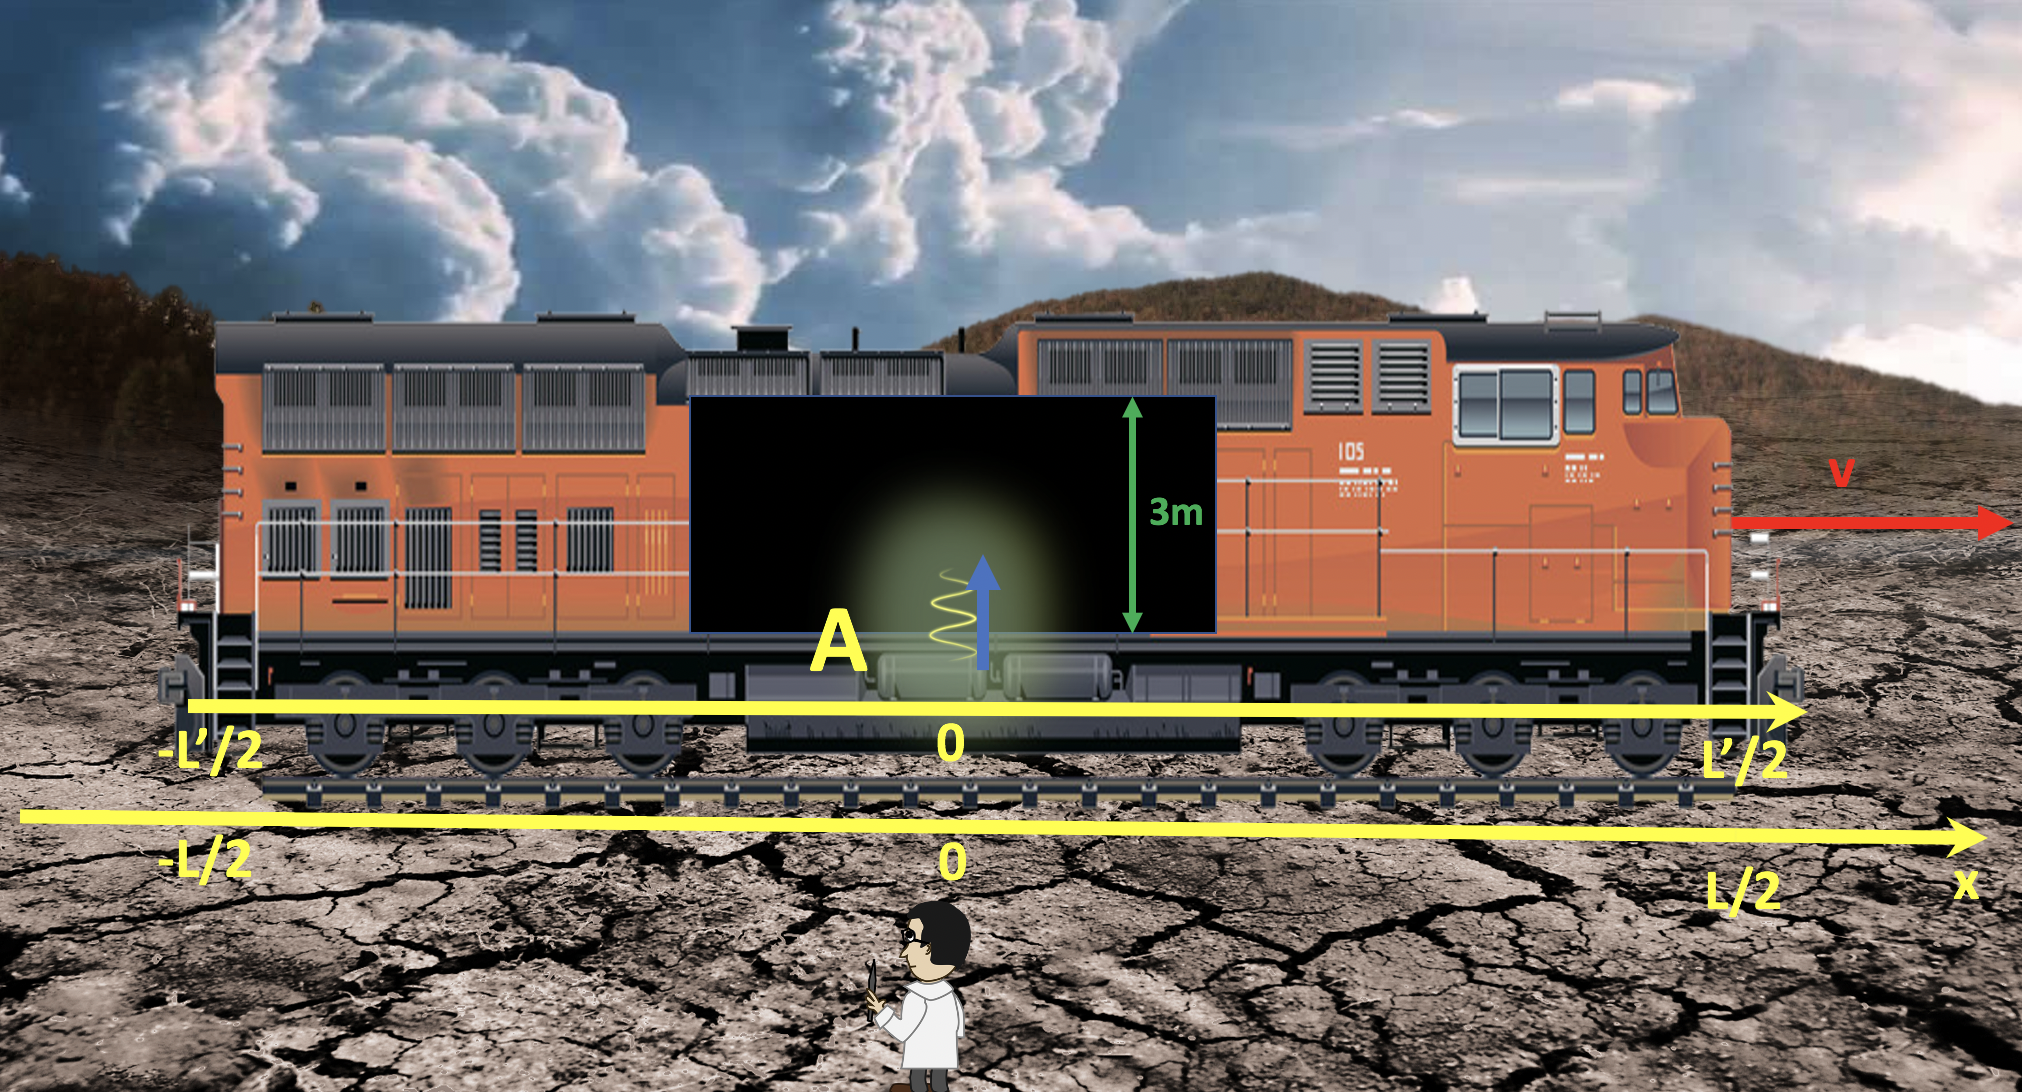
\includegraphics[scale=0.26]{media/eks1.png}}
Toget har en x'-akse som står fast på toget, origo ($x'=0$) er midtpunktet på toget som beveger seg mot høyre med fart $v$. Bakken har en x-akse. En sensor gjør at i det origo på x'-aksen er i samme x-posisjon som origo på x-aksen på bakken (i bildet over), så startes stoppeklokken både på toget (tid $t'$) og på bakken (tid $t$) med $t=t'=0$. Samtidig sendes et lysstråle rett oppover i toget fra origo på x'-asken (togets midtpunkt)
Vi kaller utsendelsen av lysstrålen for event A.\\
{\tiny Figurene i dette dokumentet er png-er fra hiclipart.com som har blitt satt sammen og mikset}
}{SIDE 9/19/39}

\fullframe{eks3}{eks2}{eks4}{0}{\small
\centerline{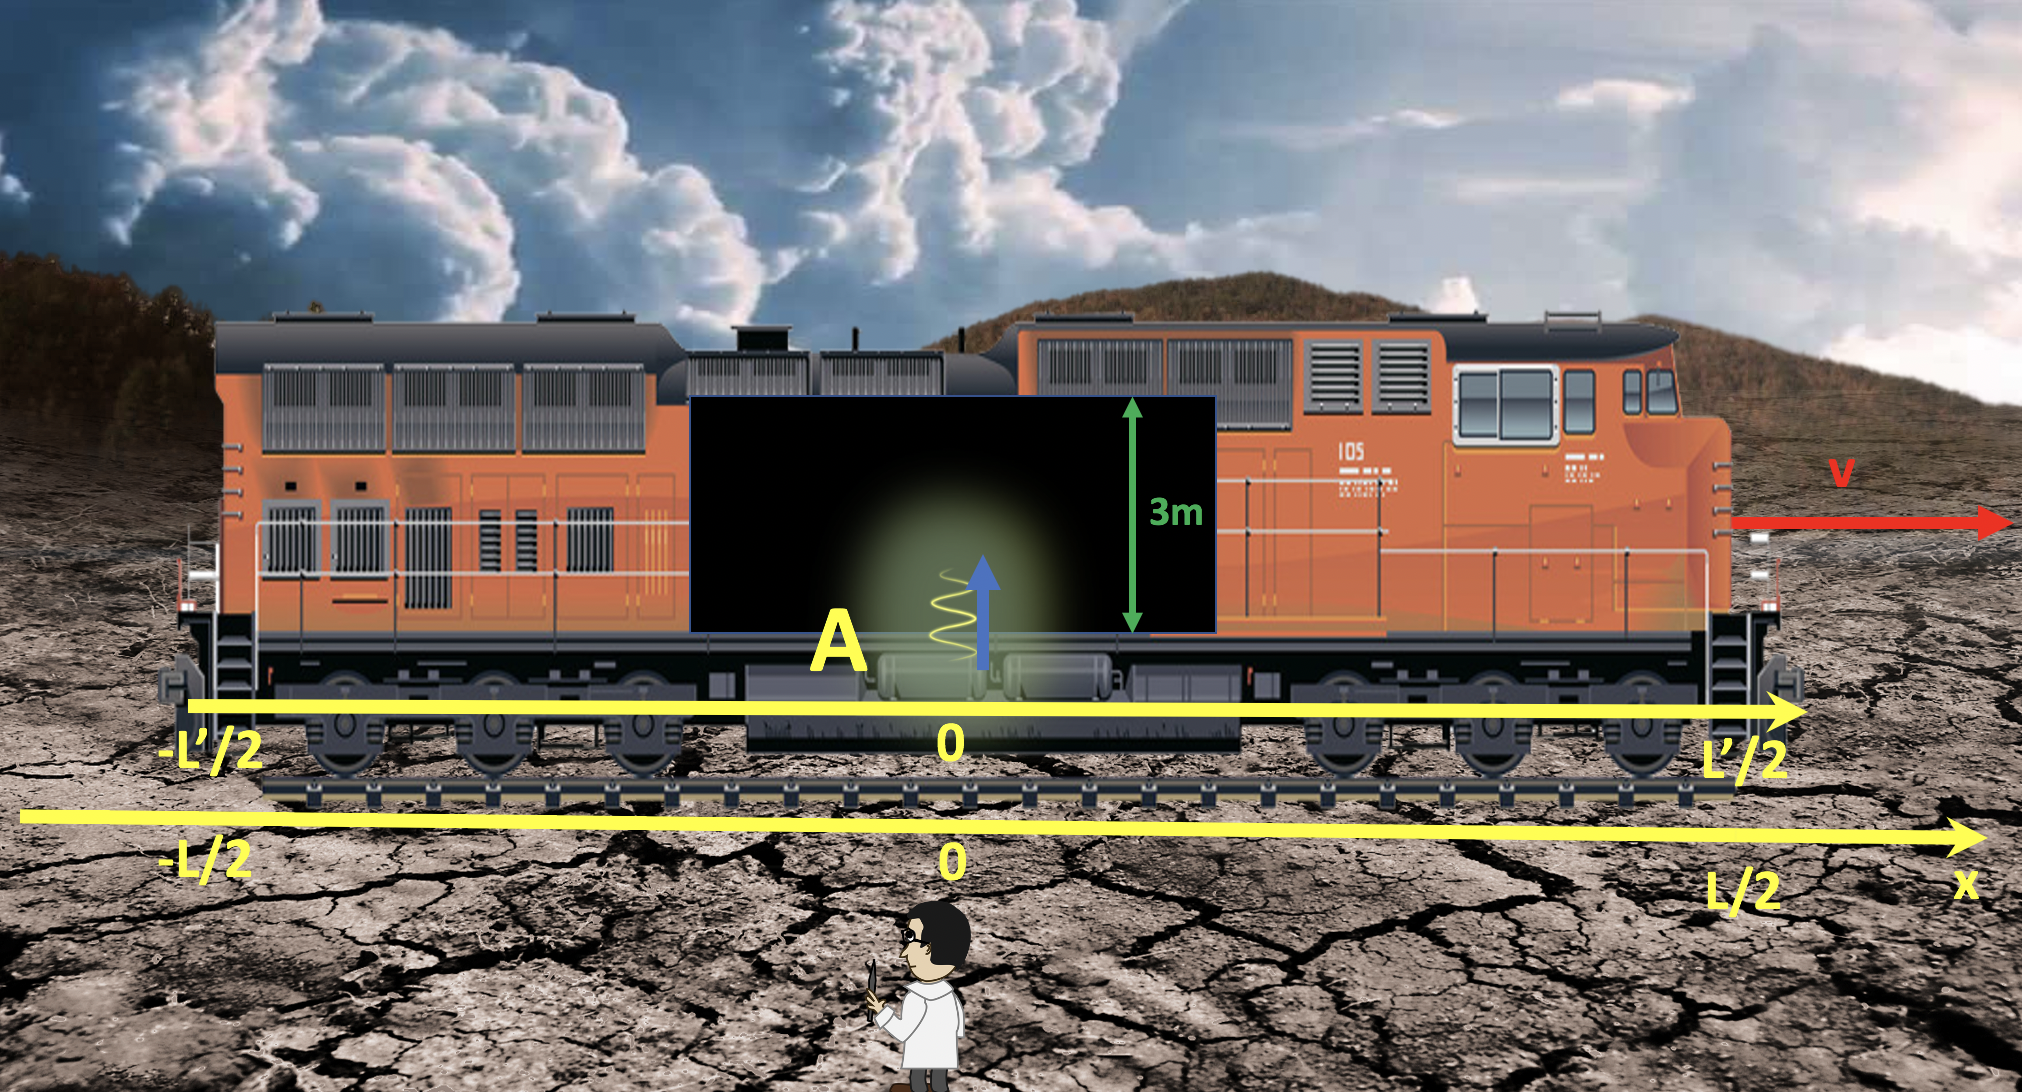
\includegraphics[scale=0.26]{media/eks1.png}}
{\footnotesize Merk at event A her også kan kalles {\bf origoeventet}. Origoeventet er et event som skjer i origo på begge aksene. Dvs. det skjer når origo i de to aksene er på samme x-koordinat slik at en observatør som er i origo i begge systemer kan treffes fysisk. Origoeventet skjer på $x=x'=0$. Normalt (slik som her) så bruker vi også origoeventet til å starte klokkene slik at ogsa $t=t'=0$ i dette eventet. Vi ser for oss at vi har en stoppeklokke som står i origo i hvert av systemene. I det origo i begge systemer berører hverandre, nullstilles begge klokkene og de begynner å gå.}
}{SIDE 10/19/39}


\fullframe{eks4}{eks3}{eks5}{0}{
\centerline{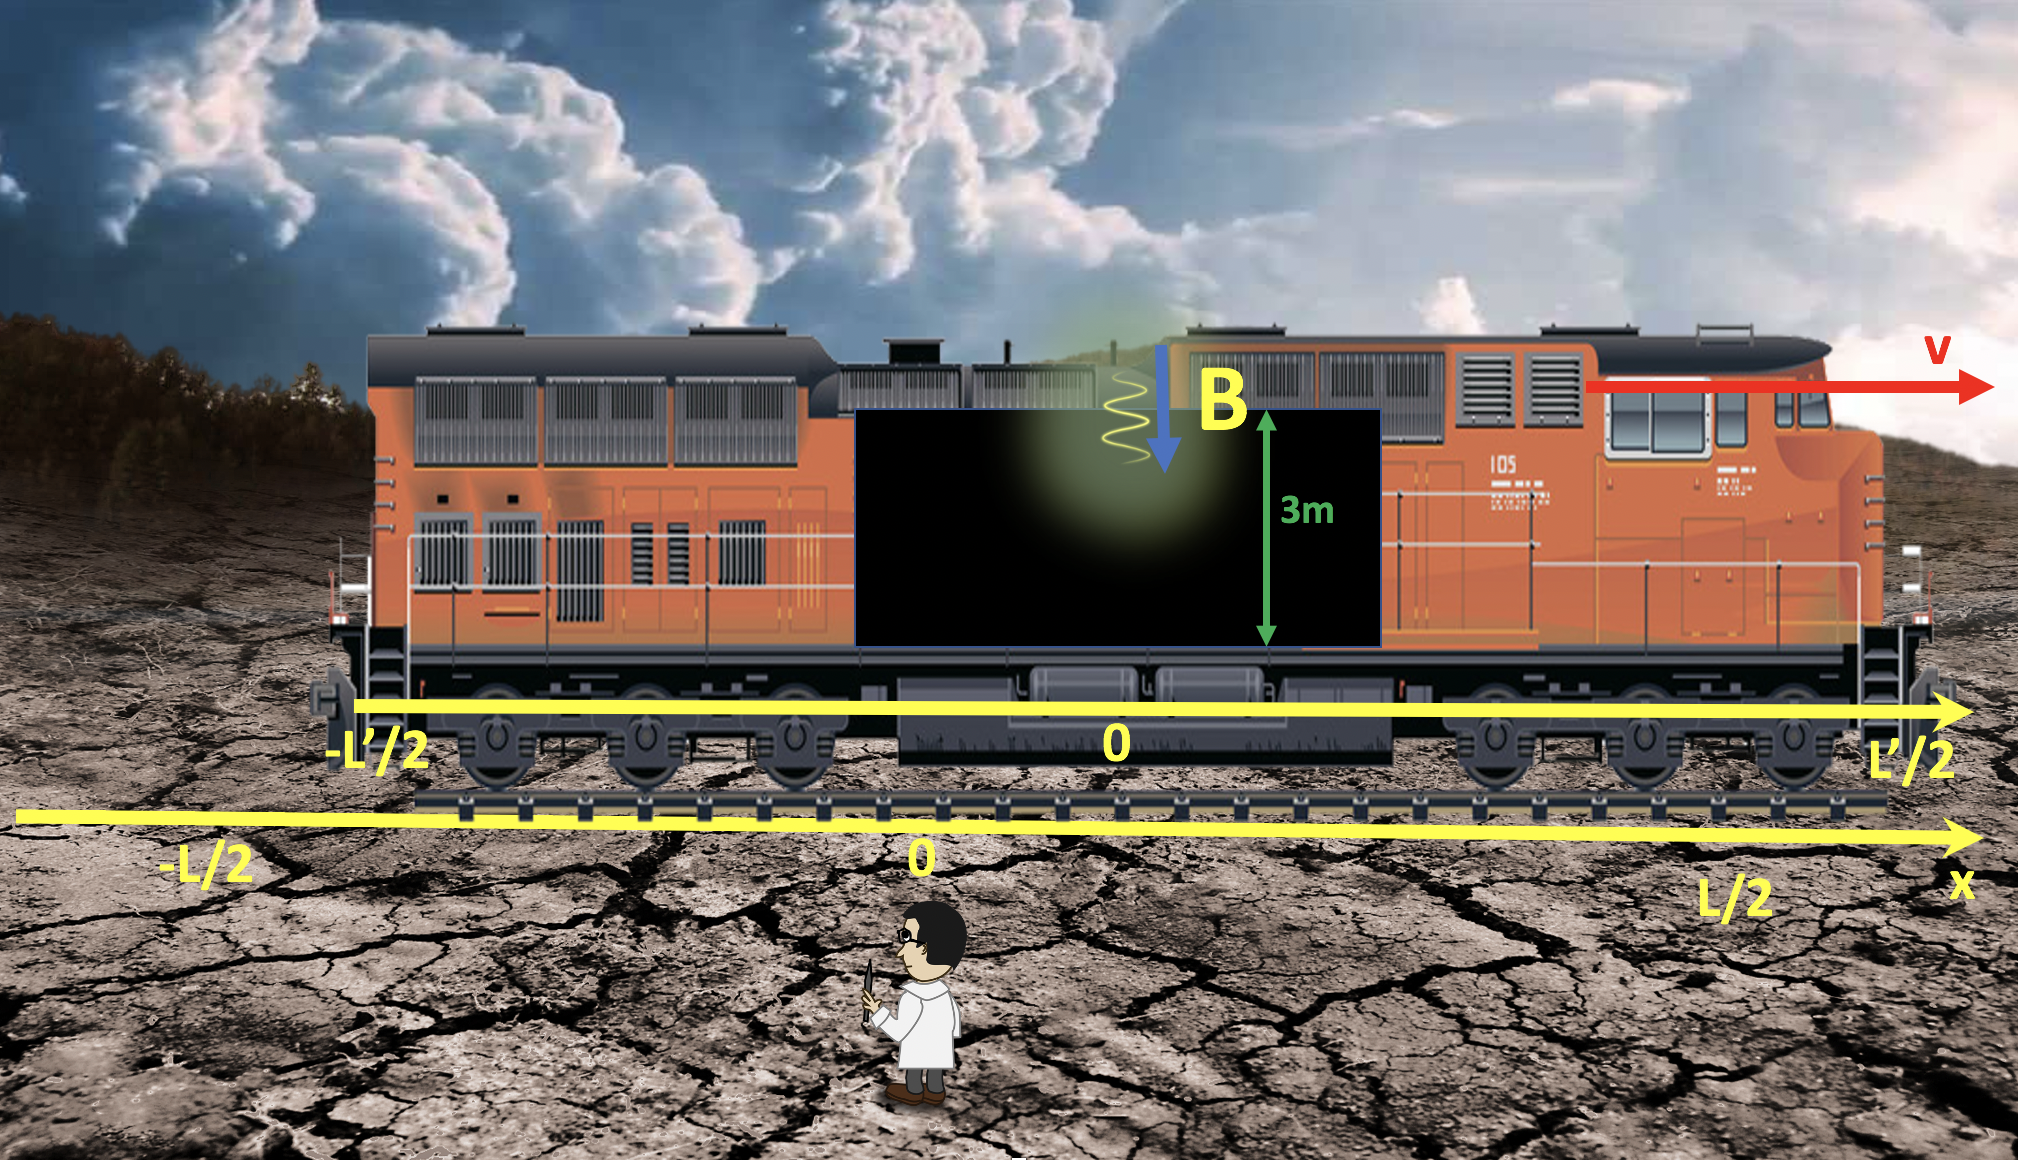
\includegraphics[scale=0.26]{media/eks2.png}}
Et speil i taket gjør at lysstrålen reflekteres tilbake igjen når den treffer taket. Dette kalles event B. I labsystemet, så har toget beveget seg en liten strekning til høyre for origo på x-aksen. Merk at x'-aksen sitter fast på toget og flytter seg med toget.
}{SIDE 11/19/39}

\fullframe{eks5}{eks4}{eks6}{0}{
\centerline{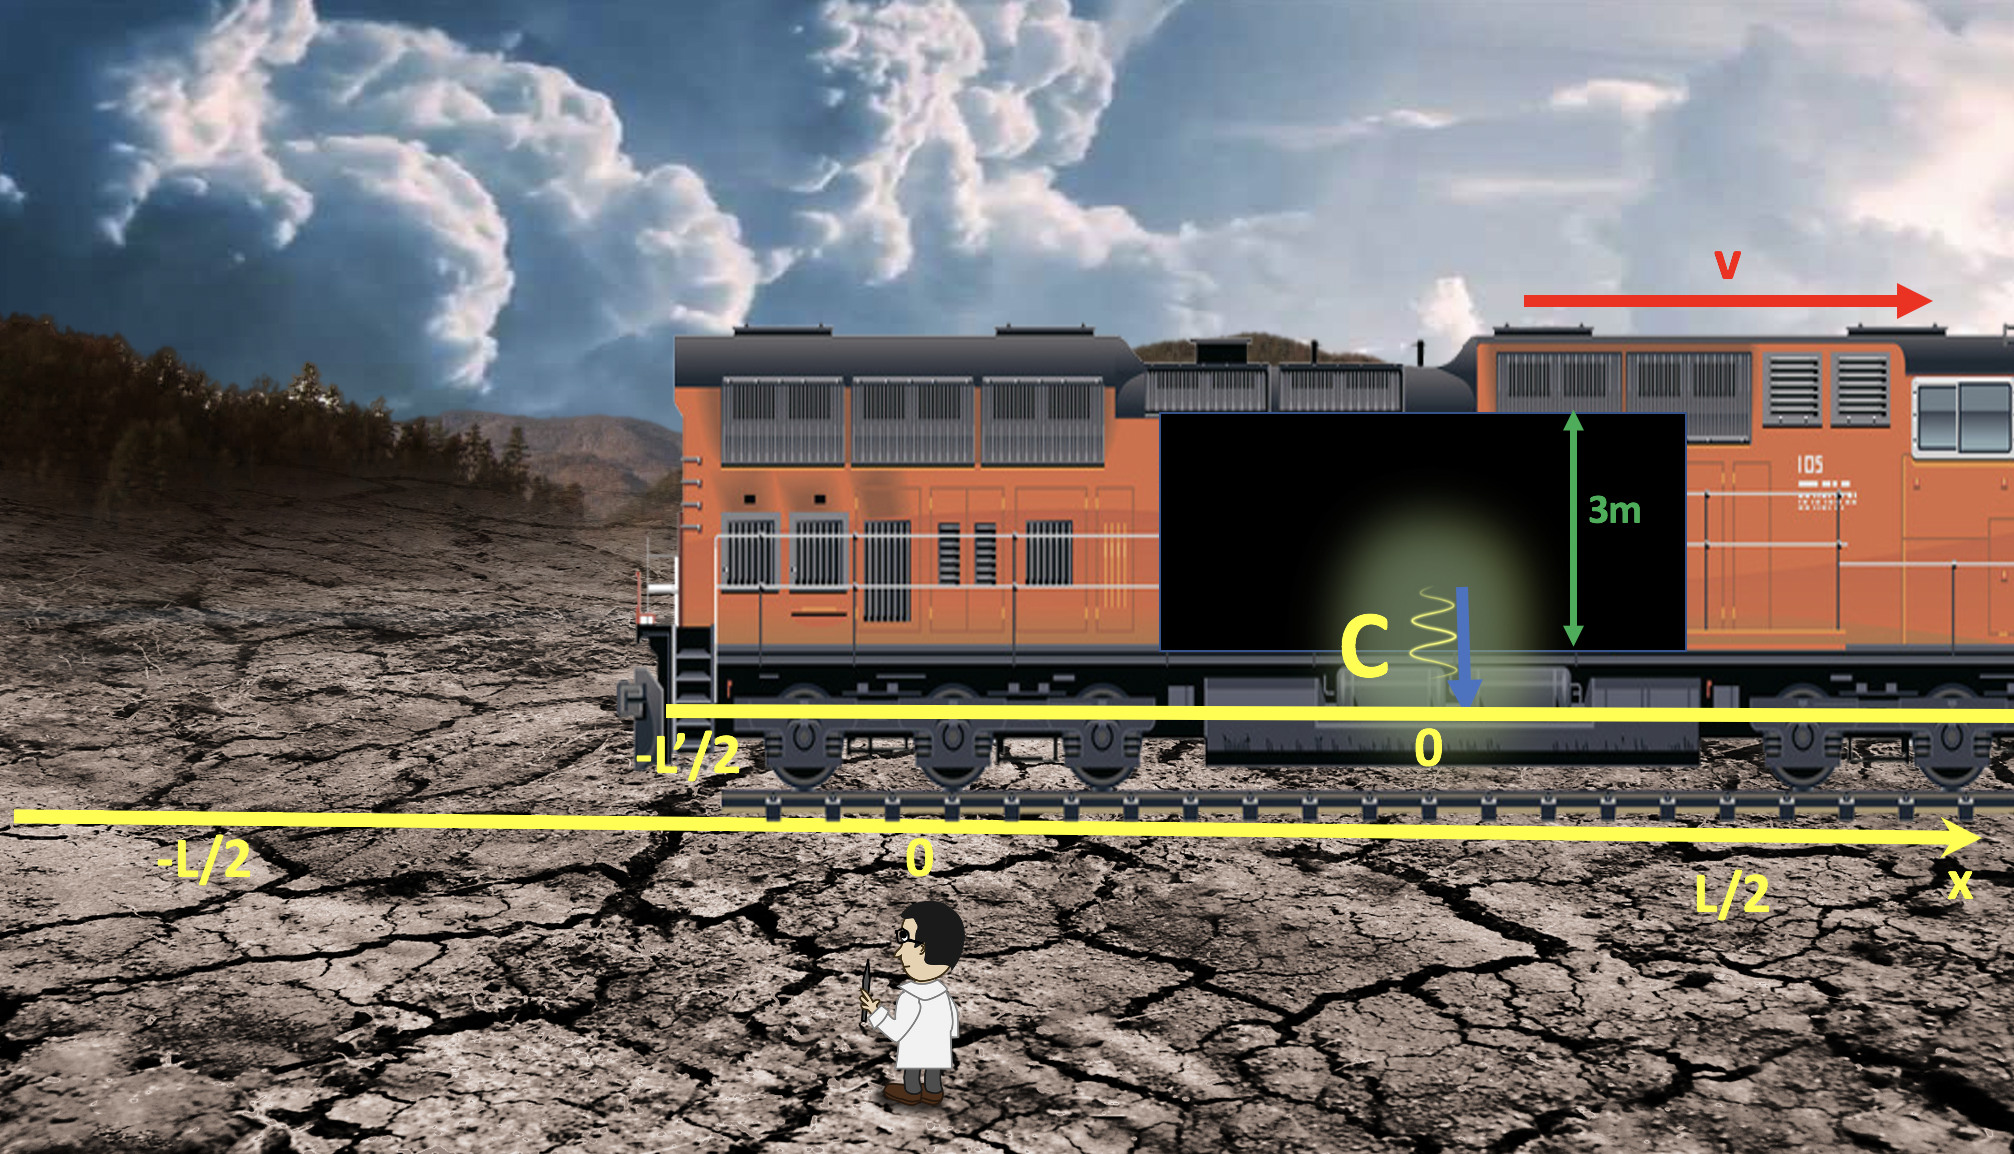
\includegraphics[scale=0.26]{media/eks3.png}}
Event C er at lysstrålen kommer tilbake til gulvet i toget (i origo på x'-aksen i togsystemet). Da har toget flyttet seg enda lenger bortover langs x-aksen i labsystemet. {\bf Du får nå oppgitt at midtpunktet (origo på x'-aksen) har flyttet seg 8 meter langs x-aksen i labsystemet siden event A skjedde.}.
}{SIDE 12/19/39}

\fullframe{eks6}{eks5}{eks8}{0}{
Når du får en slik problemstilling er det første du {\bf alltid} skal gjøre, å sette opp posisjoner og tidspunkter for alle eventer i alle referansesystemer. Hvis noen er ukjente så lar du de stå åpne. Ta et stykke papir, og skriv nå opp $x_A$, $x_B$, $x_A'$, $x_B'$, $t_A$, $t_B$, $t_A'$, $t_B'$ med tall for de som du nå har nok informasjon til å kjenne. Vi skal bruke {\bf meter} som enhet, alle tall skal angies i meter. Ikke gå videre før du har alle tallene som du kan finne enkelt uten regning.
}{SIDE 13/19/39}

\fullframe{eks8}{eks6}{eks9}{0}{\large
Fikk du:
\begin{align*}
x_A&=0, &x_B&=4m, &x_C&=8m\\
x'_A&=0, &x'_B&=0, &x'_C&=0\\
t_A&=0, &t_B&=?, &t_C&=?\\
t_A'&=0, &t_B'&=3m, &t_C'&=6m
\end{align*}
{\bf Forstår du hvorfor det blir sånn?} Hvis du har den minste tvil, se på \href{https://www.uio.no/studier/emner/matnat/astro/AST2000/h20/undervisningsmateriell/interaktive-forelesningsnotater/2a/videoer/video2a_4.mp4}{denne videoen for forklaringer}.
}{SIDE 14/19/39}


\fullframenotxt{eks9}{eks8}{eks10}{0}{
  Hva så med tidspunktene $t_B$ og $t_C$ i bakkesystemet? Kan vi bruke invarians av tidromsintervallet? Isåfall hvordan? \hyperlink{eks9_b}{\pagebutton{Jeg har tenkt litt over det og har kanskje en ide}}
  \textcolor{white}{
Vi vet hvor langt det er mellom f.eks. event A og C i både tid og rom i togsystemet, enig? Dvs. vi kjenner både $\Delta x_\mathrm{AC}'$ og $\Delta t_\mathrm{AC}'$ i togsystemet, dermed kan vi vel enkelt finne $\Delta s' = \sqrt{(\Delta t')^2-(\Delta x')^2}$? {høres rimlig ut det ja...}\\
Kan du regne ut tidromsintervallet mellom event A og event C i meter?{ok, done...}\\
Fikk du $\Delta s' = \sqrt{(6\m)^2-0^2}=6\m$? {det må det bli!}\\
Vi kjenner altså tidromsintervallet mellom eventene! I bakkesystemet kjenner vi kun den romlige avstanden mellom A og C, men ikke tidsintervallet. Kan du bruke invarians av tidromsintervallet til å finne $t_C'$?}
}{SIDE 15/19/39}

\fullframenotxt{eks9_b}{eks8}{eks10}{0}{
Hva så med tidspunktene $t_B$ og $t_C$ i bakkesystemet? Kan vi bruke invarians av tidromsintervallet? Isåfall hvordan? \pagebutton{Jeg har tenkt litt over det og har kanskje en ide}
Vi vet hvor langt det er mellom f.eks. event A og C i både tid og rom i togsystemet, enig? Dvs. vi kjenner både $\Delta x_\mathrm{AC}'$ og $\Delta t_\mathrm{AC}'$ i togsystemet, dermed kan vi vel enkelt finne $\Delta s' = \sqrt{(\Delta t')^2-(\Delta x')^2}$? \hyperlink{eks9_c}{\pagebutton{høres rimlig ut det ja...}}
\textcolor{white}{
Kan du regne ut tidromsintervallet mellom event A og event C i meter? {ok, done...}{0}\\
Fikk du $\Delta s' = \sqrt{(6\m)^2-0^2}=6\m$? {det må det bli!}\\
Vi kjenner altså tidromsintervallet mellom eventene! I bakkesystemet kjenner vi kun den romlige avstanden mellom A og C, men ikke tidsintervallet. Kan du bruke invarians av tidromsintervallet til å finne $t_C'$?}
}{SIDE 15/19/39}

\fullframenotxt{eks9_c}{eks8}{eks10}{0}{
Hva så med tidspunktene $t_B$ og $t_C$ i bakkesystemet? Kan vi bruke invarians av tidromsintervallet? Isåfall hvordan? \pagebutton{Jeg har tenkt litt over det og har kanskje en ide}
Vi vet hvor langt det er mellom f.eks. event A og C i både tid og rom i togsystemet, enig? Dvs. vi kjenner både $\Delta x_\mathrm{AC}'$ og $\Delta t_\mathrm{AC}'$ i togsystemet, dermed kan vi vel enkelt finne $\Delta s' = \sqrt{(\Delta t')^2-(\Delta x')^2}$? \pagebutton{høres rimlig ut det ja...}
Kan du regne ut tidromsintervallet mellom event A og event C i meter? \hyperlink{eks9_d}{\pagebutton{ok, done...}}
\textcolor{white}{
Fikk du $\Delta s' = \sqrt{(6\m)^2-0^2}=6\m$? {det må det bli!}\\
Vi kjenner altså tidromsintervallet mellom eventene! I bakkesystemet kjenner vi kun den romlige avstanden mellom A og C, men ikke tidsintervallet. Kan du bruke invarians av tidromsintervallet til å finne $t_C'$?}
}{SIDE 15/19/39}

\fullframenotxt{eks9_d}{eks8}{eks10}{0}{
Hva så med tidspunktene $t_B$ og $t_C$ i bakkesystemet? Kan vi bruke invarians av tidromsintervallet? Isåfall hvordan? \pagebutton{Jeg har tenkt litt over det og har kanskje en ide}
Vi vet hvor langt det er mellom f.eks. event A og C i både tid og rom i togsystemet, enig? Dvs. vi kjenner både $\Delta x_\mathrm{AC}'$ og $\Delta t_\mathrm{AC}'$ i togsystemet, dermed kan vi vel enkelt finne $\Delta s' = \sqrt{(\Delta t')^2-(\Delta x')^2}$? \pagebutton{høres rimlig ut det ja...}
Kan du regne ut tidromsintervallet mellom event A og event C i meter? \pagebutton{ok, done...}
Fikk du $\Delta s' = \sqrt{(6\m)^2-0^2}=6\m$? \hyperlink{eks9_e}{\pagebutton{det må det bli!}}
\textcolor{white}{
Vi kjenner altså tidromsintervallet mellom eventene! I bakkesystemet kjenner vi kun den romlige avstanden mellom A og C, men ikke tidsintervallet. Kan du bruke invarians av tidromsintervallet til å finne $t_C'$?}
}{SIDE 15/19/39}

\fullframetxt{eks9_e}{eks8}{eks10}{0}{La meg tenke og regne bittelitt her...}{
Hva så med tidspunktene $t_B$ og $t_C$ i bakkesystemet? Kan vi bruke invarians av tidromsintervallet? Isåfall hvordan? \pagebutton{Jeg har tenkt litt over det og har kanskje en ide}
Vi vet hvor langt det er mellom f.eks. event A og C i både tid og rom i togsystemet, enig? Dvs. vi kjenner både $\Delta x_\mathrm{AC}'$ og $\Delta t_\mathrm{AC}'$ i togsystemet, dermed kan vi vel enkelt finne $\Delta s' = \sqrt{(\Delta t')^2-(\Delta x')^2}$? \pagebutton{høres rimlig ut det ja...}
Kan du regne ut tidromsintervallet mellom event A og event C i meter? \pagebutton{ok, done...}
Fikk du $\Delta s' = \sqrt{(6\m)^2-0^2}=6\m$? \pagebutton{det må det bli!}
Vi kjenner altså tidromsintervallet mellom eventene! I bakkesystemet kjenner vi kun den romlige avstanden mellom A og C, men ikke tidsintervallet. Kan du bruke invarians av tidromsintervallet til å finne $t_C'$?
}{SIDE 15/19/39}

\fullframetxt{eks10}{eks9}{eks11}{1}{OK!}{
Vi vet at $\Delta s$ er den samme i begge referanssystemer, altså den er 6m. Altså har vi også at
\[
\Delta s^2=\Delta t^2 - \Delta x^2=(t_C-t_A)^2-(x_C-x_A)^2
\]
Men her er vel alt unntatt $t_C$ kjent? Løser vi for $t_C$ her får vi
\[
t_C=\sqrt{(8\m)^2+(6\m)^2}=10\m
\]
Enig?
}{SIDE 16/19/39}

\fullframetwonotxt{eks11}{eks10}{eks11x}{0}{\footnotesize
Ofte er dette eneste måte å løse problemet på, men i dette tilfellet her finnes det en annen som gir litt mer innsikt i problemstillingen. Prøv å tegne hele lysstrålen fra A til C i labsystemet. Sett mål på alle lengder på tegningen.\\
\hyperlink{eks11_b}{\pagebutton{\footnotesize Ok, jeg har gjort det}}
\textcolor{white}{
Ble den slik?\\
\vspace*{5cm}
der høyden er 3m?\\
{\footnotesize Jepp!}\\
Streken fra A til B er jo avstanden som lyset har tilbakelagt fra A til B. Kan du bruke geometri på figuren til å finne}\\
\vspace*{4cm}
}
{\textcolor{white}{
\footnotesize
denne avstanden? Tilsvarende for A til C?\\
{\footnotesize Ok, jeg har regnet}\\
Ble det $\sqrt{(4\m)^2+(3\m)^2}=5m$ for både A til B og B til C? Dermed har lyset totalt tilbakelagt en avstand på $2\sqrt{(4\m)^2+(3\m)^2}=10m$ fra A til C?\\
{\footnotesize Enig!}\\
Men hvor lang tid bruker lys på å bevege seg en avstand 10m? (angi svaret i meter)\\
{\footnotesize Ja, det må vel være...}\\
...10 meter det? Et tidsintervall på 10 meter var jo definert som tiden lyset bruker på å tilbakelegge 10 m, det var slik vi regnet om tidsintervaller til meter. Men da har vi også funnet hvor lang tid det tar fra event A til event C i labsystemet, nøyaktig samme svar som vi fikk med å regne invarians av tidromsintervallet på forrige side. Alt er konsistent!}
\vspace*{4cm}
}{SIDE 17/19/39}


\fullframetwonotxt{eks11_b}{eks10}{eks11x}{0}{\footnotesize
Ofte er dette eneste måte å løse problemet på, men i dette tilfellet her finnes det en annen som gir litt mer innsikt i problemstillingen. Prøv å tegne hele lysstrålen fra A til C i labsystemet. Sett mål på alle lengder på tegningen.\\
\pagebutton{\footnotesize Ok, jeg har gjort det}
Ble den slik?
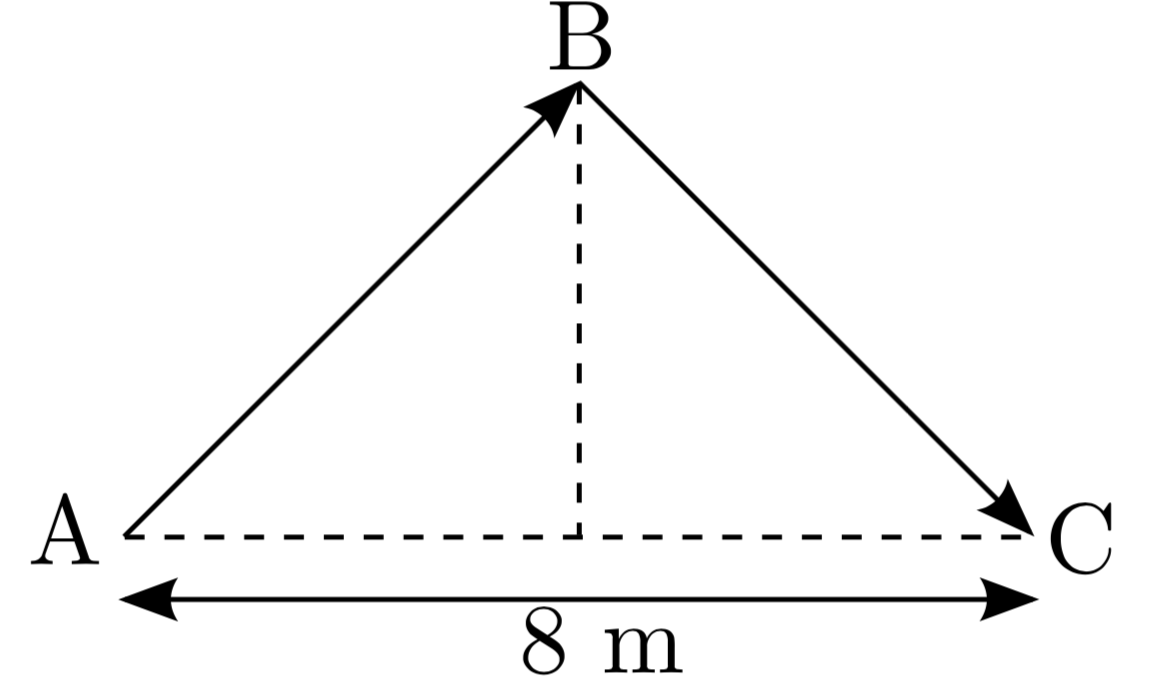
\includegraphics[scale=0.25]{media/triangle.png}\\
der høyden er 3m?\\
\hyperlink{eks11_c}{\pagebutton{\footnotesize Jepp!}}
\textcolor{white}{
Streken fra A til B er jo avstanden som lyset har tilbakelagt fra A til B. Kan du bruke geometri på figuren til å finne}\\
\vspace*{4cm}
}
{\textcolor{white}{\footnotesize
denne avstanden? Tilsvarende for A til C?\\
{\footnotesize Ok, jeg har regnet}\\
Ble det $\sqrt{(4\m)^2+(3\m)^2}=5m$ for både A til B og B til C? Dermed har lyset totalt tilbakelagt en avstand på $2\sqrt{(4\m)^2+(3\m)^2}=10m$ fra A til C?\\
{\footnotesize Enig!}\\
Men hvor lang tid bruker lys på å bevege seg en avstand 10m? (angi svaret i meter)\\
{\footnotesize Ja, det må vel være...}\\
...10 meter det? Et tidsintervall på 10 meter var jo definert som tiden lyset bruker på å tilbakelegge 10 m, det var slik vi regnet om tidsintervaller til meter. Men da har vi også funnet hvor lang tid det tar fra event A til event C i labsystemet, nøyaktig samme svar som vi fikk med å regne invarians av tidromsintervallet på forrige side. Alt er konsistent!}
\vspace*{4cm}
}{SIDE 17/19/39}


\fullframetwonotxt{eks11_c}{eks10}{eks11x}{0}{\footnotesize
Ofte er dette eneste måte å løse problemet på, men i dette tilfellet her finnes det en annen som gir litt mer innsikt i problemstillingen. Prøv å tegne hele lysstrålen fra A til C i labsystemet. Sett mål på alle lengder på tegningen.\\
\pagebutton{\footnotesize Ok, jeg har gjort det}
Ble den slik?
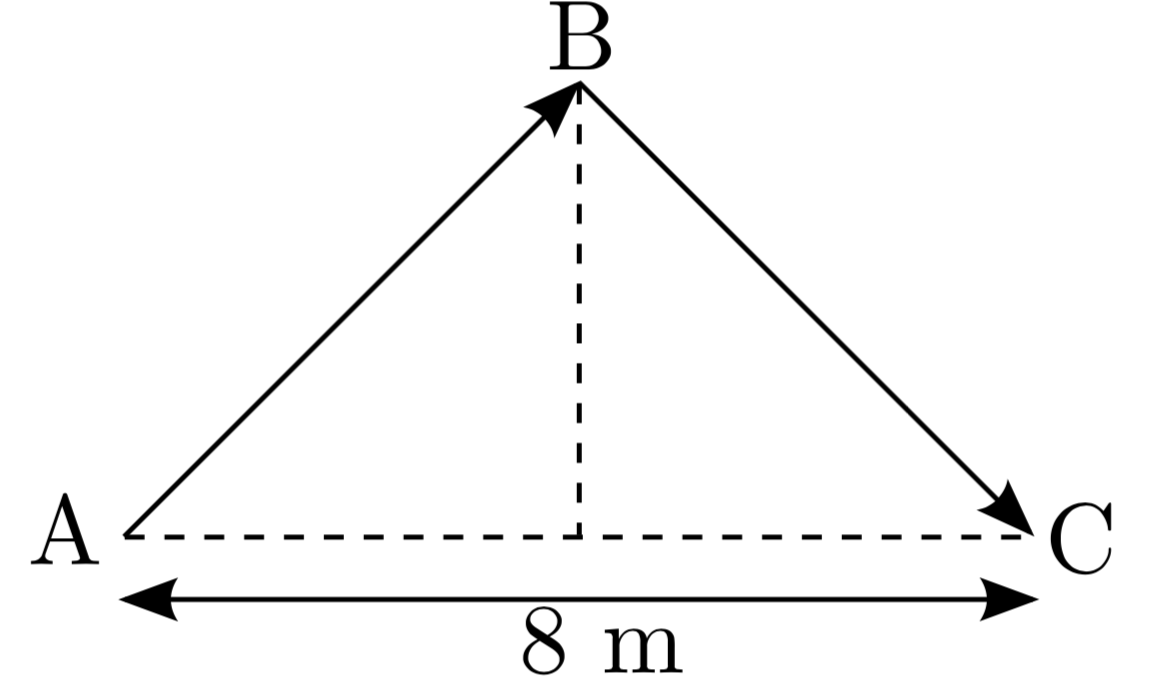
\includegraphics[scale=0.25]{media/triangle.png}\\
der høyden er 3m?\\
\pagebutton{\footnotesize Jepp!}
Streken fra A til B er jo avstanden som lyset har tilbakelagt fra A til B. Kan du bruke geometri på figuren til å finne\\
\vspace*{4cm}
}
{\footnotesize
denne avstanden? Tilsvarende for A til C?\\
\hyperlink{eks11_d}{\pagebutton{\footnotesize Ok, jeg har regnet}}
\textcolor{white}{
Ble det $\sqrt{(4\m)^2+(3\m)^2}=5m$ for både A til B og B til C? Dermed har lyset totalt tilbakelagt en avstand på $2\sqrt{(4\m)^2+(3\m)^2}=10m$ fra A til C?\\
{\footnotesize Enig!}\\
Men hvor lang tid bruker lys på å bevege seg en avstand 10m? (angi svaret i meter)\\
{\footnotesize Ja, det må vel være...}\\
...10 meter det? Et tidsintervall på 10 meter var jo definert som tiden lyset bruker på å tilbakelegge 10 m, det var slik vi regnet om tidsintervaller til meter. Men da har vi også funnet hvor lang tid det tar fra event A til event C i labsystemet, nøyaktig samme svar som vi fikk med å regne invarians av tidromsintervallet på forrige side. Alt er konsistent!}
\vspace*{4cm}
}{SIDE 17/19/39}


\fullframetwonotxt{eks11_d}{eks10}{eks11x}{0}{\footnotesize
Ofte er dette eneste måte å løse problemet på, men i dette tilfellet her finnes det en annen som gir litt mer innsikt i problemstillingen. Prøv å tegne hele lysstrålen fra A til C i labsystemet. Sett mål på alle lengder på tegningen.\\
\pagebutton{\footnotesize Ok, jeg har gjort det}
Ble den slik?
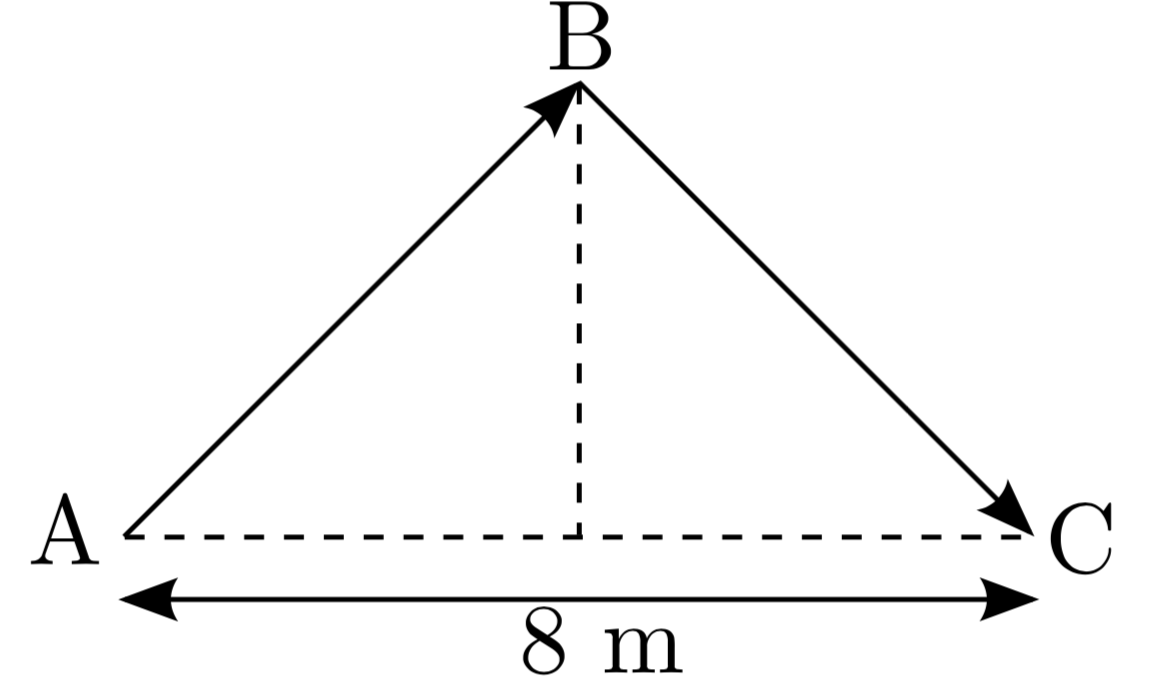
\includegraphics[scale=0.25]{media/triangle.png}\\
der høyden er 3m?\\
\pagebutton{\footnotesize Jepp!}
Streken fra A til B er jo avstanden som lyset har tilbakelagt fra A til B. Kan du bruke geometri på figuren til å finne\\
\vspace*{4cm}
}
{\footnotesize
denne avstanden? Tilsvarende for A til C?\\
\pagebutton{\footnotesize Ok, jeg har regnet}
Ble det $\sqrt{(4\m)^2+(3\m)^2}=5m$ for både A til B og B til C? Dermed har lyset totalt tilbakelagt en avstand på $2\sqrt{(4\m)^2+(3\m)^2}=10m$ fra A til C?\\
\hyperlink{eks11_e}{\pagebutton{\footnotesize Enig!}}
\textcolor{white}{
Men hvor lang tid bruker lys på å bevege seg en avstand 10m? (angi svaret i meter)\\
{\footnotesize Ja, det må vel være...}\\
...10 meter det? Et tidsintervall på 10 meter var jo definert som tiden lyset bruker på å tilbakelegge 10 m, det var slik vi regnet om tidsintervaller til meter. Men da har vi også funnet hvor lang tid det tar fra event A til event C i labsystemet, nøyaktig samme svar som vi fikk med å regne invarians av tidromsintervallet på forrige side. Alt er konsistent!}
\vspace*{4cm}
}{SIDE 17/19/39}


\fullframetwonotxt{eks11_e}{eks10}{eks11x}{0}{\footnotesize
Ofte er dette eneste måte å løse problemet på, men i dette tilfellet her finnes det en annen som gir litt mer innsikt i problemstillingen. Prøv å tegne hele lysstrålen fra A til C i labsystemet. Sett mål på alle lengder på tegningen.\\
\pagebutton{\footnotesize Ok, jeg har gjort det}
Ble den slik?
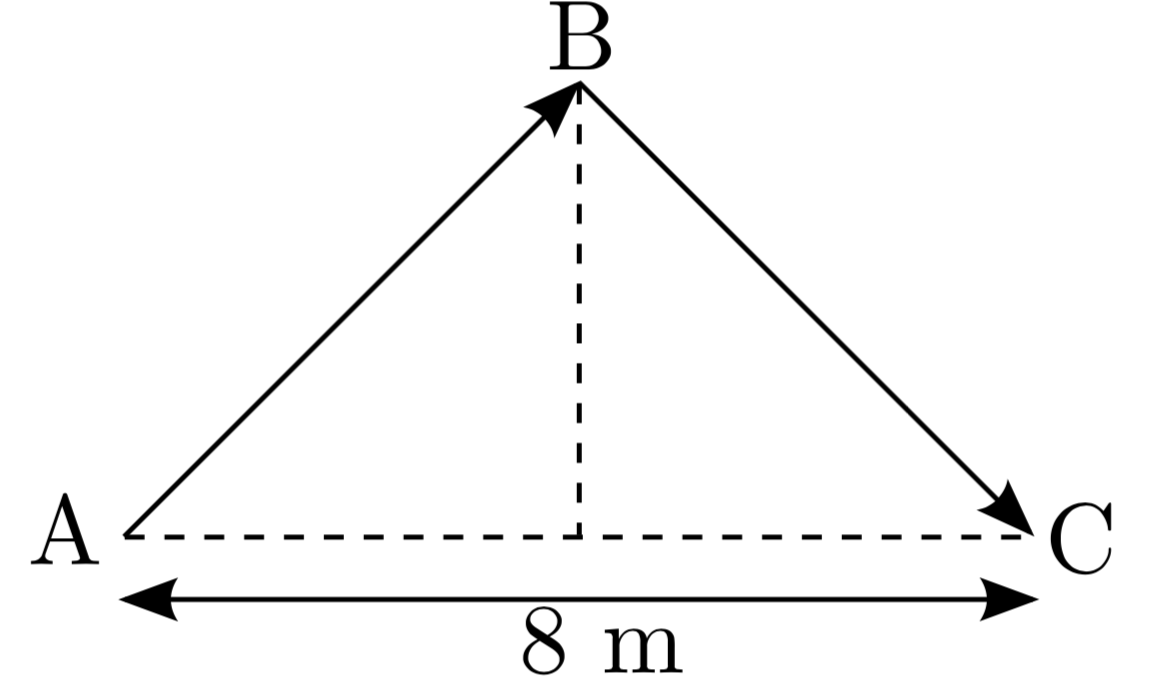
\includegraphics[scale=0.25]{media/triangle.png}\\
der høyden er 3m?\\
\pagebutton{\footnotesize Jepp!}
Streken fra A til B er jo avstanden som lyset har tilbakelagt fra A til B. Kan du bruke geometri på figuren til å finne\\
\vspace*{4cm}
}
{\footnotesize
denne avstanden? Tilsvarende for A til C?\\
\pagebutton{\footnotesize Ok, jeg har regnet}
Ble det $\sqrt{(4\m)^2+(3\m)^2}=5m$ for både A til B og B til C? Dermed har lyset totalt tilbakelagt en avstand på $2\sqrt{(4\m)^2+(3\m)^2}=10m$ fra A til C?\\
\pagebutton{\footnotesize Enig!}
Men hvor lang tid bruker lys på å bevege seg en avstand 10m? (angi svaret i meter)\\
\hyperlink{eks11_f}{\pagebutton{\footnotesize Ja, det må vel være...}}
\textcolor{white}{
...10 meter det? Et tidsintervall på 10 meter var jo definert som tiden lyset bruker på å tilbakelegge 10 m, det var slik vi regnet om tidsintervaller til meter. Men da har vi også funnet hvor lang tid det tar fra event A til event C i labsystemet, nøyaktig samme svar som vi fikk med å regne invarians av tidromsintervallet på forrige side. Alt er konsistent!}
\vspace*{4cm}
}{SIDE 17/19/39}


\fullframetwo{eks11_f}{eks10}{eks11x}{0}{\footnotesize
Ofte er dette eneste måte å løse problemet på, men i dette tilfellet her finnes det en annen som gir litt mer innsikt i problemstillingen. Prøv å tegne hele lysstrålen fra A til C i labsystemet. Sett mål på alle lengder på tegningen.\\
\pagebutton{\footnotesize Ok, jeg har gjort det}
Ble den slik?
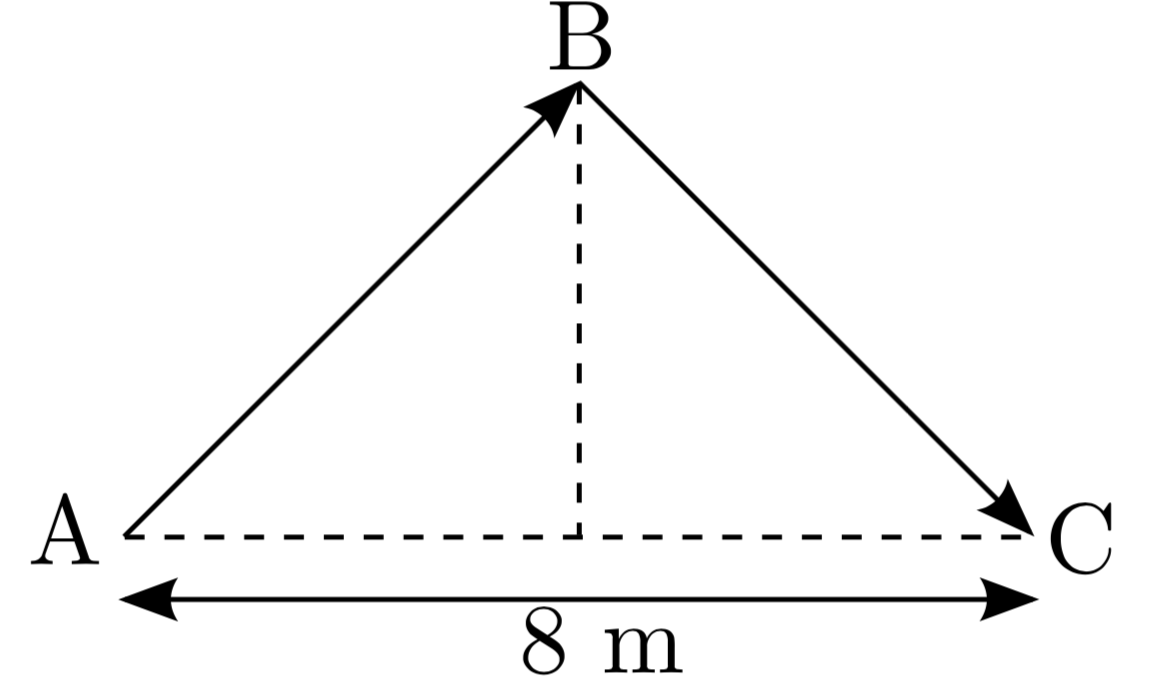
\includegraphics[scale=0.25]{media/triangle.png}\\
der høyden er 3m?\\
\pagebutton{\footnotesize Jepp!}
Streken fra A til B er jo avstanden som lyset har tilbakelagt fra A til B. Kan du bruke geometri på figuren til å finne\\
\vspace*{4cm}
}
{\footnotesize
denne avstanden? Tilsvarende for A til C?\\
\pagebutton{\footnotesize Ok, jeg har regnet}
Ble det $\sqrt{(4\m)^2+(3\m)^2}=5m$ for både A til B og B til C? Dermed har lyset totalt tilbakelagt en avstand på $2\sqrt{(4\m)^2+(3\m)^2}=10m$ fra A til C?\\
\pagebutton{\footnotesize Enig!}
Men hvor lang tid bruker lys på å bevege seg en avstand 10m? (angi svaret i meter)\\
\pagebutton{\footnotesize Ja, det må vel være...}
...10 meter det? Et tidsintervall på 10 meter var jo definert som tiden lyset bruker på å tilbakelegge 10 m, det var slik vi regnet om tidsintervaller til meter. Men da har vi også funnet hvor lang tid det tar fra event A til event C i labsystemet, nøyaktig samme svar som vi fikk med å regne invarians av tidromsintervallet på forrige side. Alt er konsistent!
\vspace*{4cm}
}{SIDE 17/19/39}












\fullframe{eks11x}{eks11}{eks12}{0}{
{\bf\Large La du merke til hvordan dette eksemplet viser direkte hvorfor lyshastighetens invarians gjør at tiden må gå forskjellig i de to referansesystemene? Dette er noe det nærmeste du kan komme å få en intuisjon for hvorfor tiden må gå forskjellig så følg nøye med:}
\begin{itemize}
\item I togsystemet går lysstrålen rett opp en avstand 3 meter fra event A til event B. Tiden mellom disse to hendelsene i toget kan altså ikke ta lenger enn 3 meter med tid.
\item I bakkesystemet ser vi at lysstrålen danner hypotenusen i en trekant og dermed får en avstand å gå på 5 meter fra den blir sendt ut i event A til den når taket i event B. Altså vil det for en observatør på bakken ta 5 meter med tid fra A til B skjer i toget. På bakken må vi altså se at det tar lenger tid mellom ting som skjer i toget fordi toget har en hastighet og at lyshastigheten er den samme for begge systemer.
\end{itemize}

}{SIDE 18/19/39}


\fullframetwo{eks12}{eks11x}{pause}{1}{\small
Vi kan bruke dette til å finne tolkninger av tidromsintervallet.
{\bf La du merke til at i togsystemet så var tidromsintervallet lik tidsintervallet mellom A og C?} Dette var fordi den romlige avstanden mellom A og C var 0, dvs. eventene A og C skjedde på samme sted i togsystemet. Derfor blir dette resultatet generelt: \textcolor{red}{For to eventer som skjer på samme posisjon i et referansesystem, så er tidromsintervallet det samme som tidsintervallet mellom disse to eventene i det referansesystemet.}
Kikk igjen på denne figuren:
\centerline{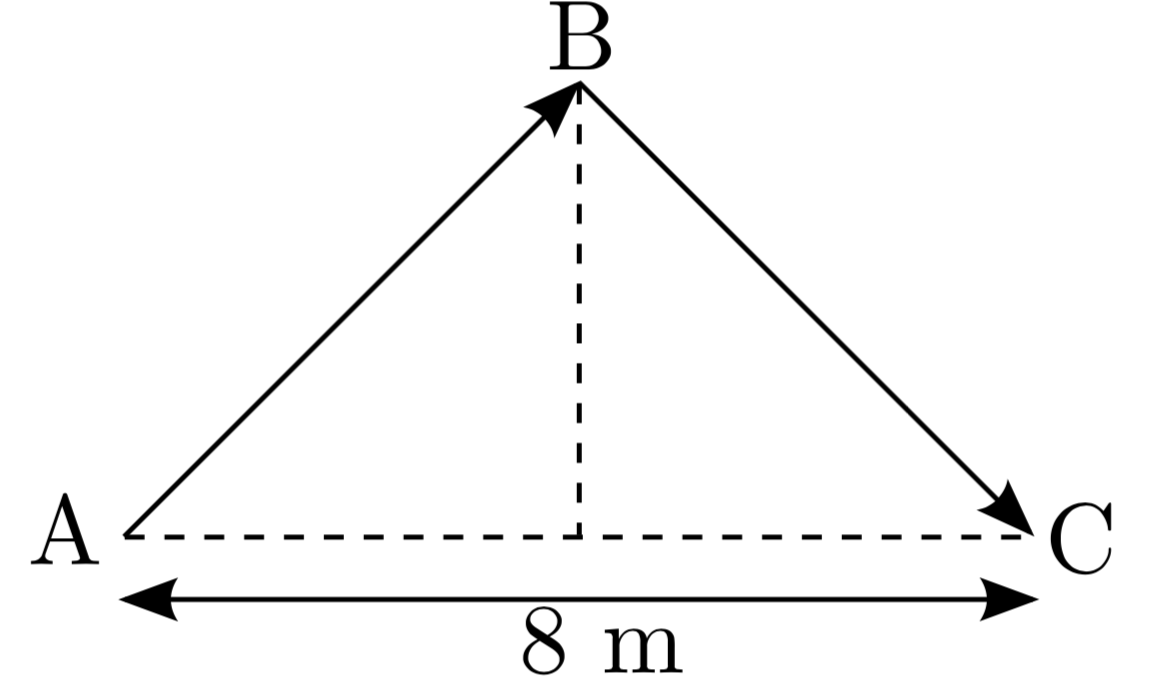
\includegraphics[scale=0.2]{media/triangle.png}}
}
{\small
{\bf kun} på trekanten til venstre fra A til B. Vi ble enige om at hypotenusen i denne trekanten er tidsintervallet mellom A og B i labsystemet. \textcolor{red}{Er du også med på at grunnlinjen her} (altså frem til midten) \textcolor{red}{er den romlige avstanden} (langs x-aksen, bevegelsesretningen) \textcolor{red}{mellom disse to eventene?} \textcolor{red}{Og høyden i denne trekanten blir da tidromsintervallet.} Dette er den generelle sammenhengen mellom disse 3 komponentene, romlig avstand, tidsintervall og tidromsintervall. \textcolor{red}{De kan representeres som sider i en rettvinklet trekant.} Siden tidsintervallet er hypotenusen kan vi slutte at dette alltid vil være større enn eller lik både tidromsintervallet og det romlige intervallet. {\bf Unntaket er når tidromsintervallet er imaginært, noe det kan være, det kommer vi tilbake til senere}.
}{SIDE 19/19/39}




{
\setbeamercolor{background canvas}{bg=cyan}
\begin{frame}
\label{pause}
\hyperlink{eks12}{\pagebutton{\small Forrige side}}
{\Large
\centerline{Kaffe allerede nå?}
\centerline{
\includegraphics[scale=4]{media/drink-coffee.png}}\\
Jepp, og ta gjerne dobbelt dose. Resten av denne forelesningen trenger {\bf din fulle konsentrasjon!} Spesielt krever den at du faktisk driver og regner litt på papir. Hvis du ikke er i humør til det nå, vent til en annen gang, ellers får du ikke noe ut av dette. Vi skal ta en liten pause underveis for at du får puste litt.
}\\
\vspace*{0.5cm}
\hyperlink{blue_nytema3}{\pagebutton{Hfuuuffffhhht (lyden av dyp innpust)...}}
\end{frame}
}


\renewcommand{\headline}{Eksempel 2}
{
\setbeamercolor{background canvas}{bg=blue}
\begin{frame}
\label{blue_nytema3}
\hyperlink{eks12}{\pagebutton{\small Forrige side}}
\nytemaside{0}
\textcolor{yellow}{Dette eksemplet har du allerede regnet på. Venninnen vår på toget og professoren som står på utsiden, og så slår lynet ned...}
\hyperlink{tog1}{\pagebutton{Sett igang!}}
\end{frame}
}


\fullframetxt{tog1}{eks12}{tog2}{0}{Ja!}{\label{eks2}
\centerline{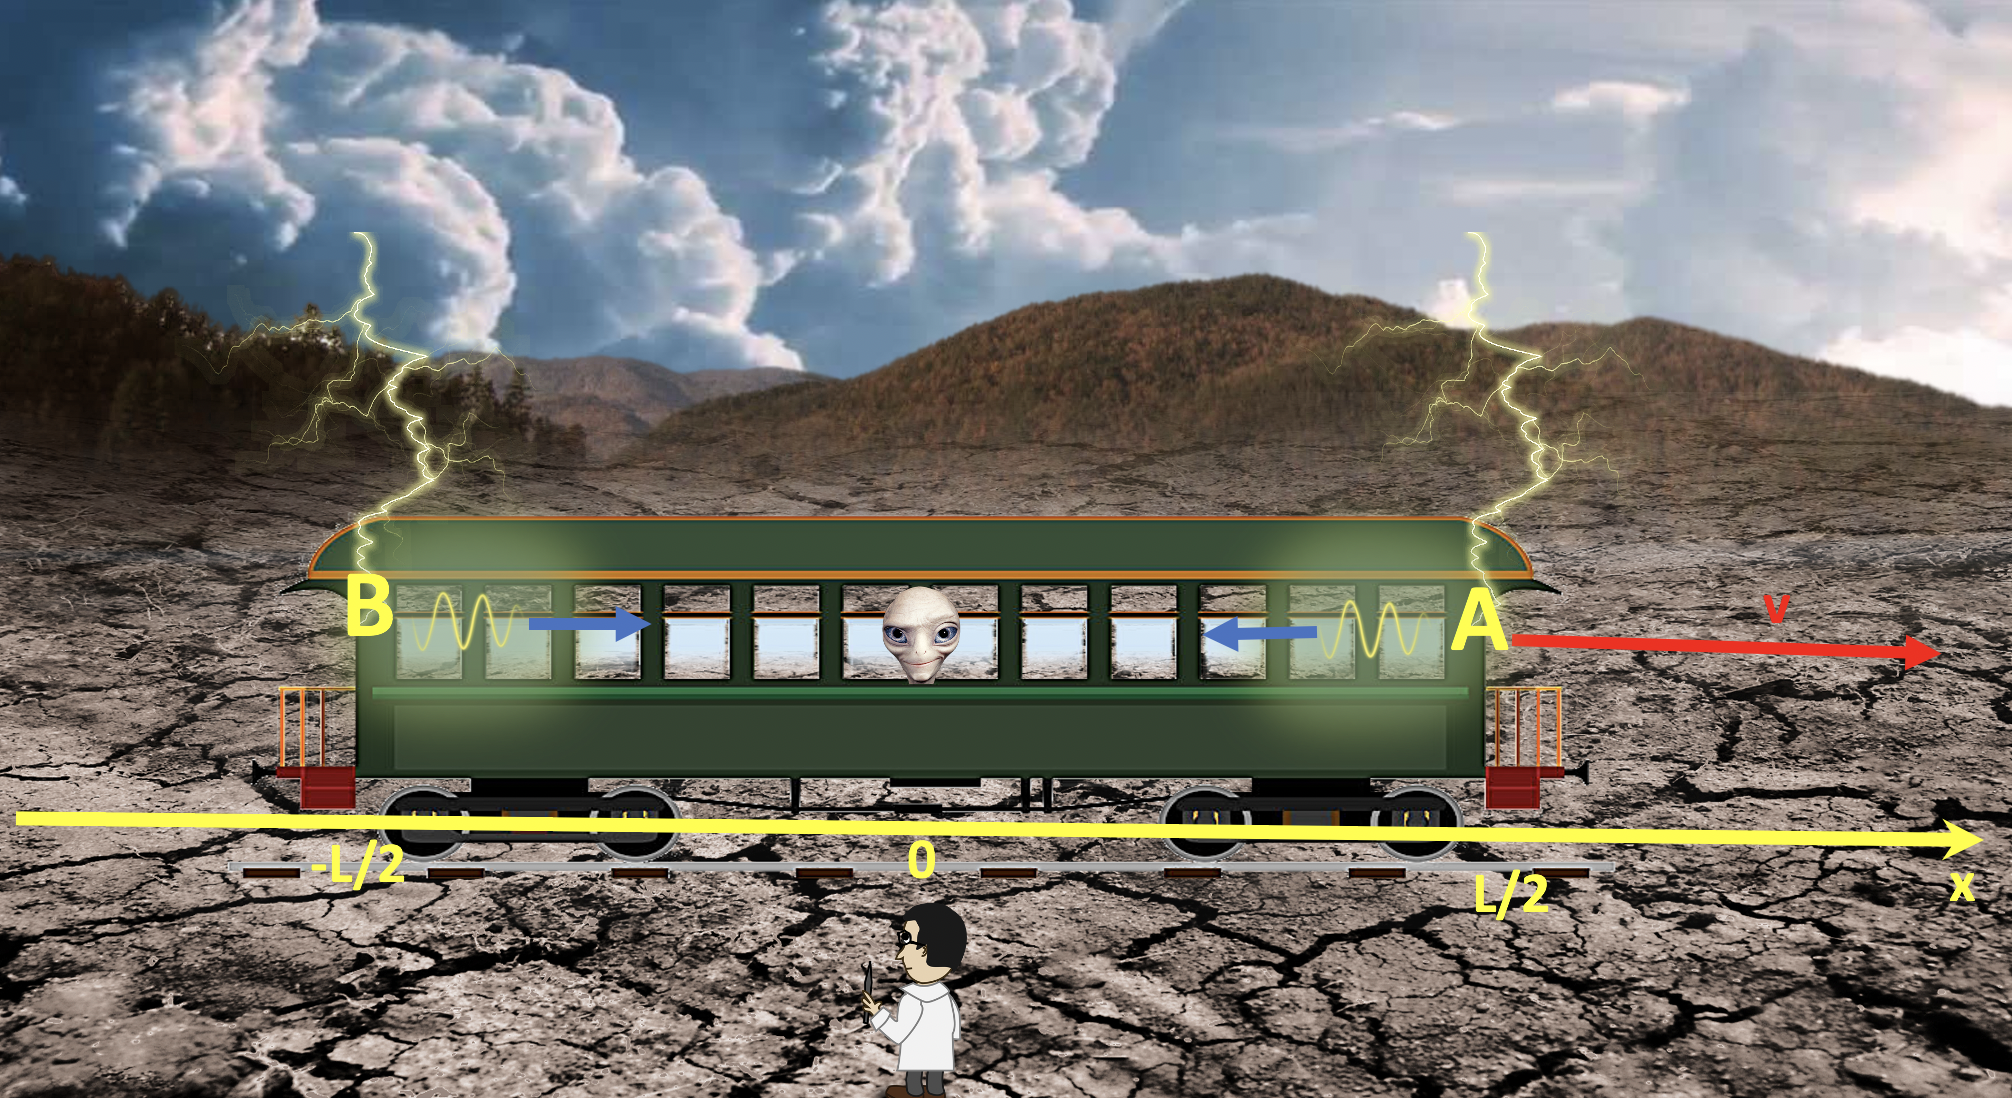
\includegraphics[scale=0.26]{media/tog1.png}}
Så var vi her igjen da! Men nå kjenner vi relativitetsteorien og skal gjøre regningene skikkelig! Og så får vi faktisk noen generelle og interessante resulter med på kjøpet. Er du klar?
}{SIDE 20/39/39}

\fullframe{tog2}{tog1}{tog3}{0}{\small
\centerline{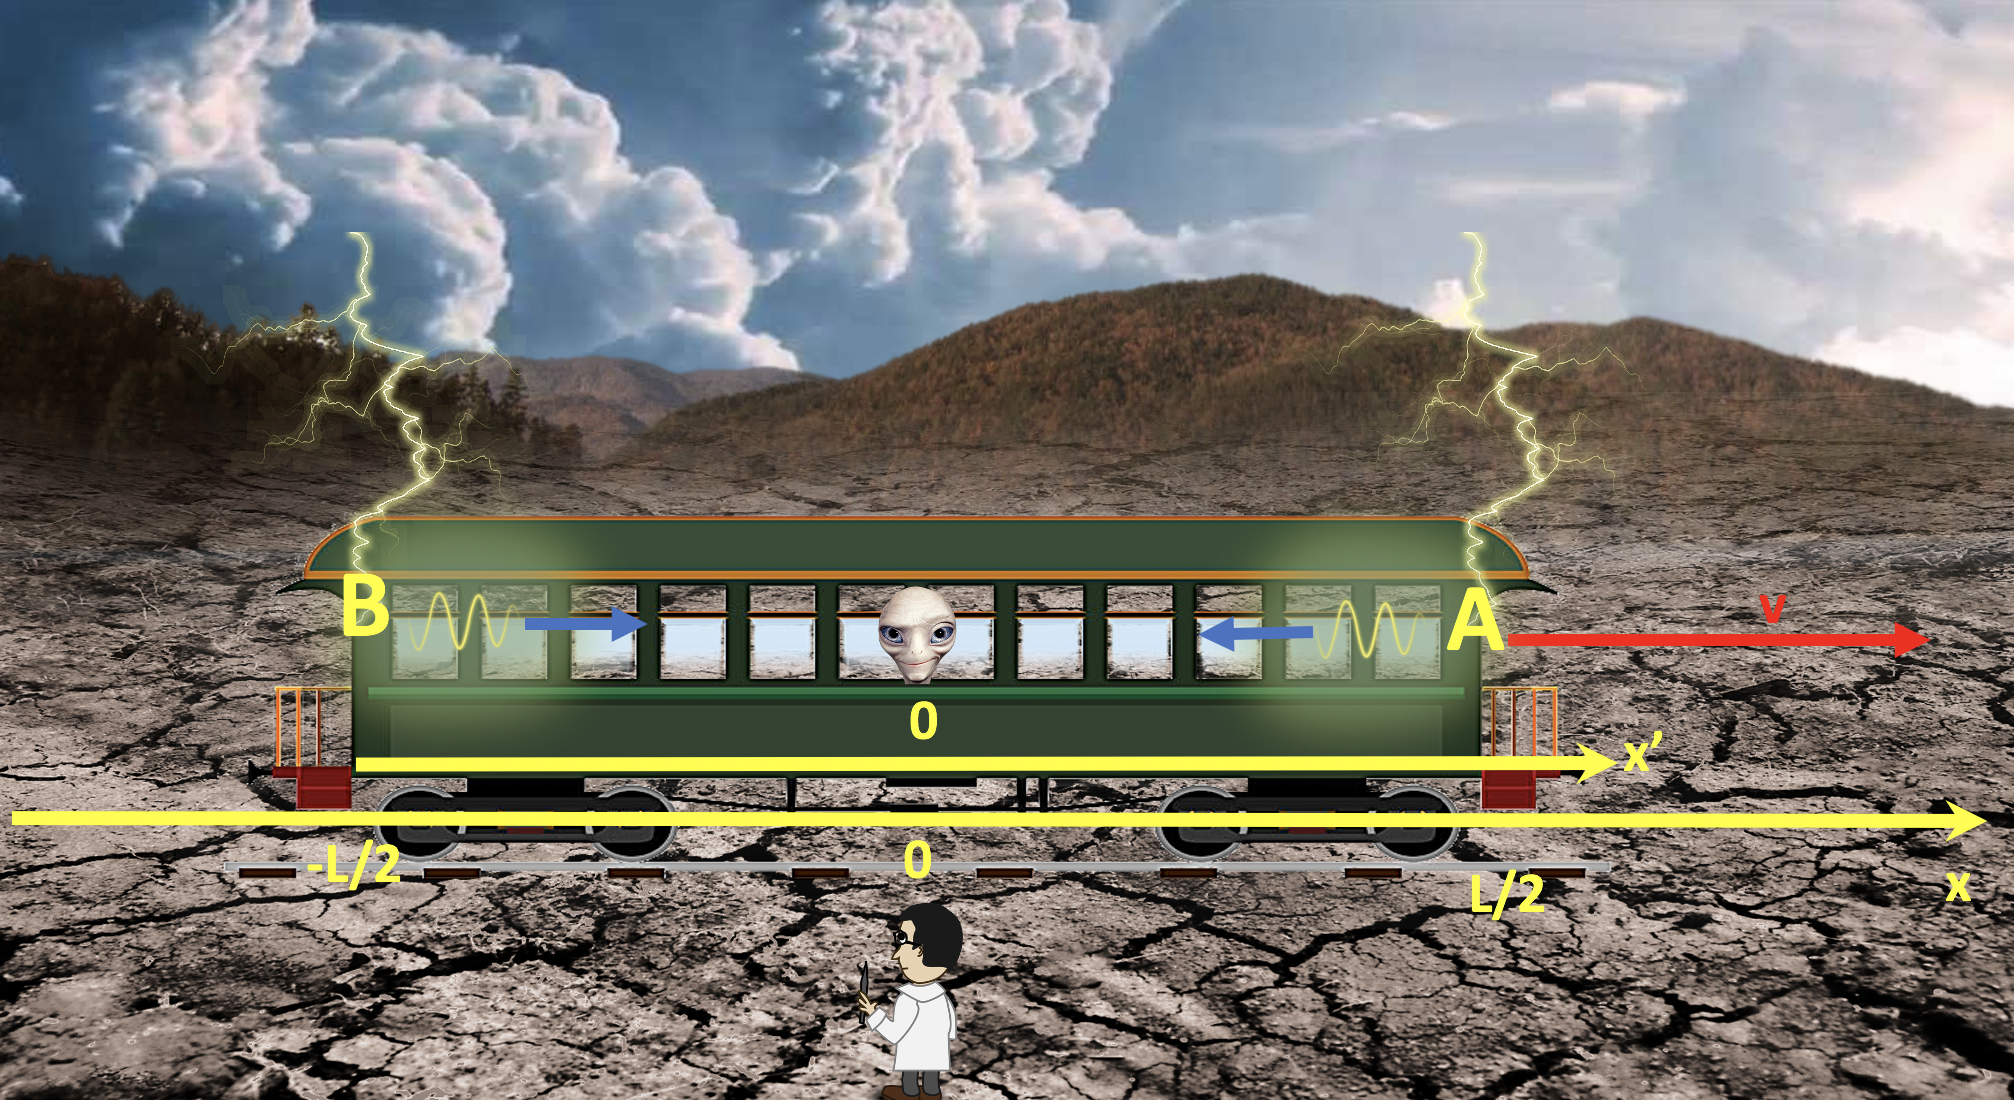
\includegraphics[scale=0.26]{media/tog6.png}}
{\footnotesize På forrige forelesning fikk vi altså til slutt vite {\bf i hvilket} referansesystem de to lynnedslagene var samtidige. De slo ned samtidig foran og bak i toget på tidspunktet da vi startet stoppeklokkene $t=0$ i labsystemet. Men i togets referansesystem var disse ikke samtidige. Det betyr at minst et av disse lynedslagene ikke skjedde i det øyeblikket origo på de to aksene var i samme posisjon, altså i det øyeblikk professoren og passasjeren hadde mulighet til raskt å håndhilse i det toget farer forbi (som også er det øyeblikket at stoppeklokkene i {\bf begge} referansesystemene ble startet på $t=t'=0$.)}
}{SIDE 21/39/39}


\fullframe{tog3}{tog2}{tog4}{0}{\small
\centerline{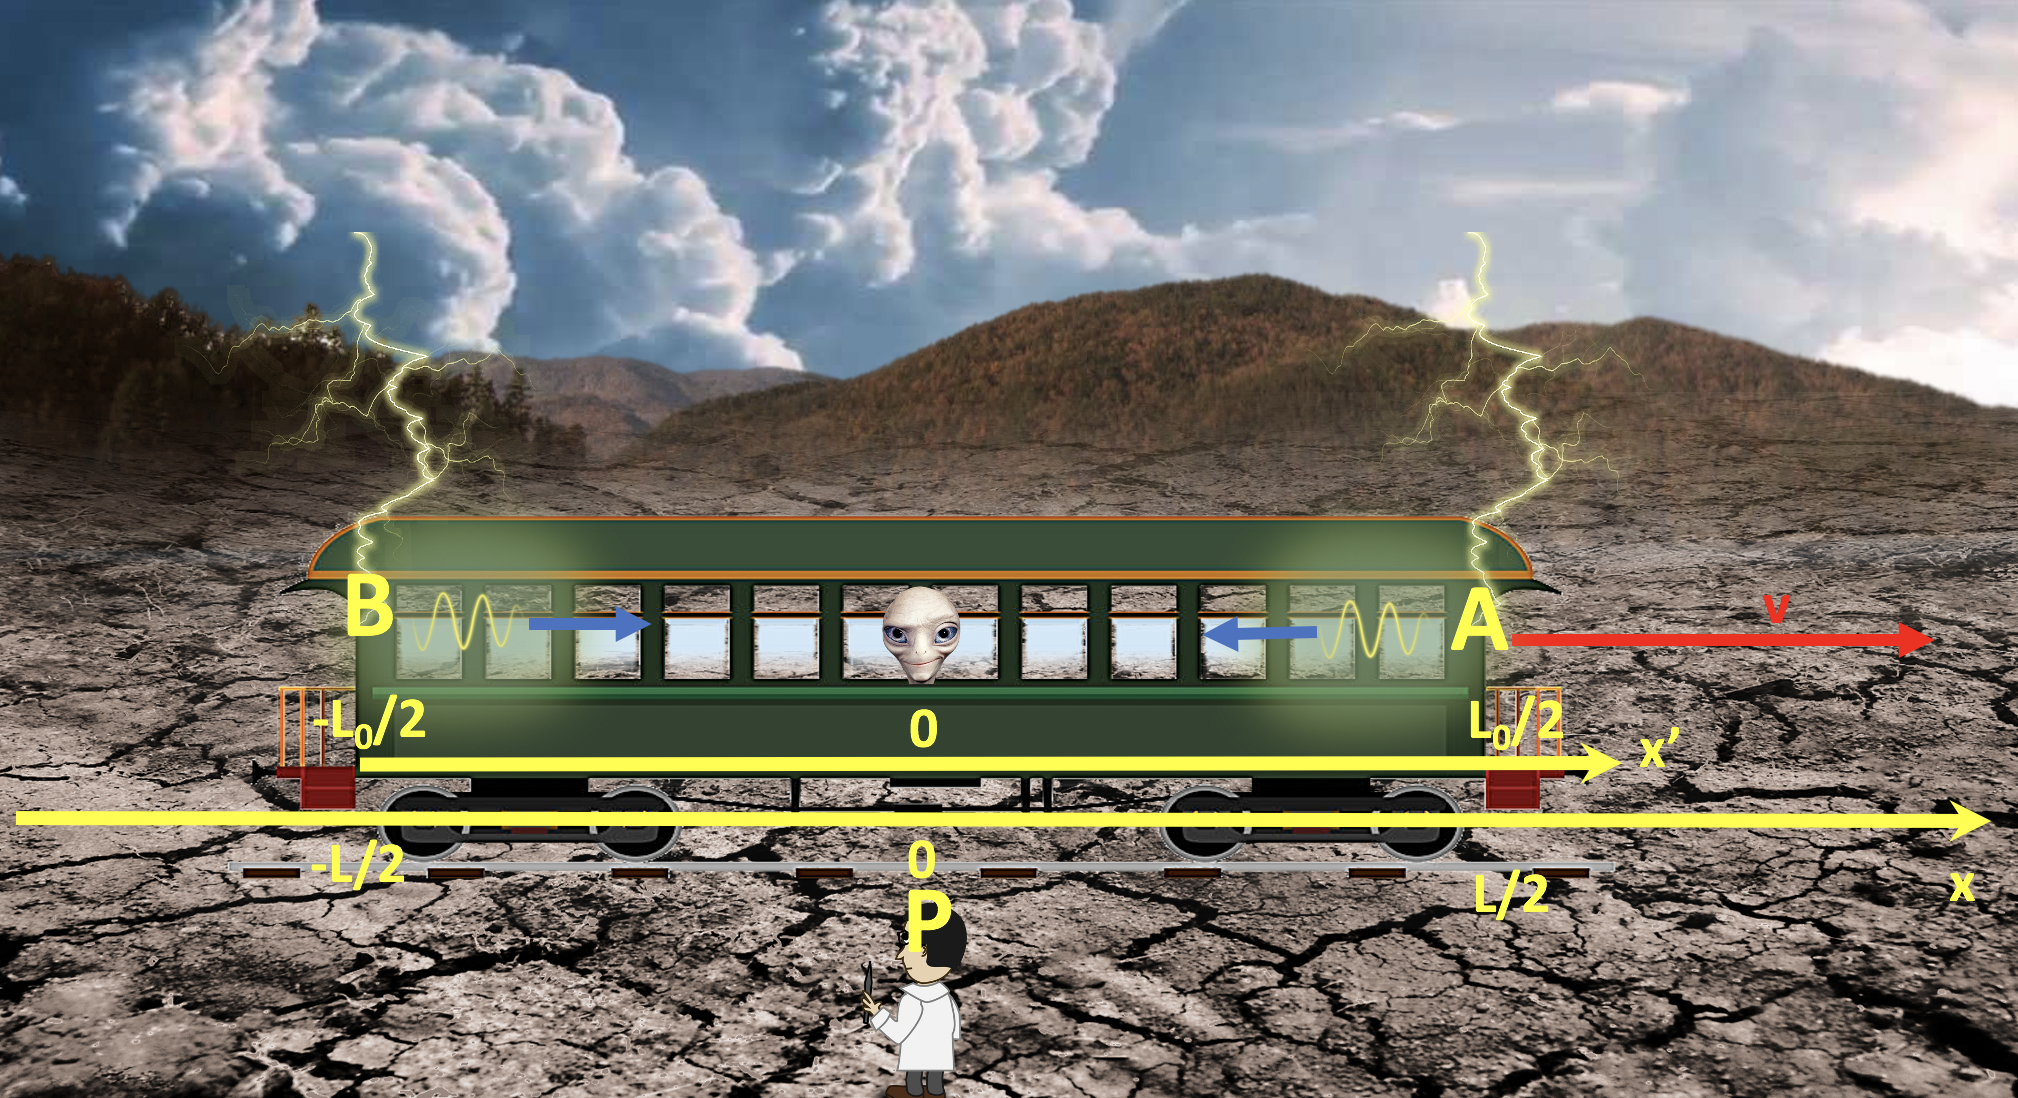
\includegraphics[scale=0.26]{media/tog7.png}}
Vi skal nå innføre nok et event, event P som er nettopp at professor O og passasjer P håndhilser, da origo i de to systemene var i samme x-posisjon og begge stoppeklokker nullstilles. Igjen så er dette {\bf origoeventet}. Vi ser eventet nå tegnet inn på bildet. Dette evente skjer altså i origo i begge systemer, som da har samme x-koordinat i dette øyeblikket. Nå som togsystemet har egen tid, må vi også åpne for at avstander kan måles forskjellig slik at vi nå kaller lengden av toget i togsystemet for $L_0$ som altså kan være forskjellige fra $L$ målt i labsystemet.
}{SIDE 22/39/39}

\fullframe{tog4}{tog3}{tog5}{0}{\small
\centerline{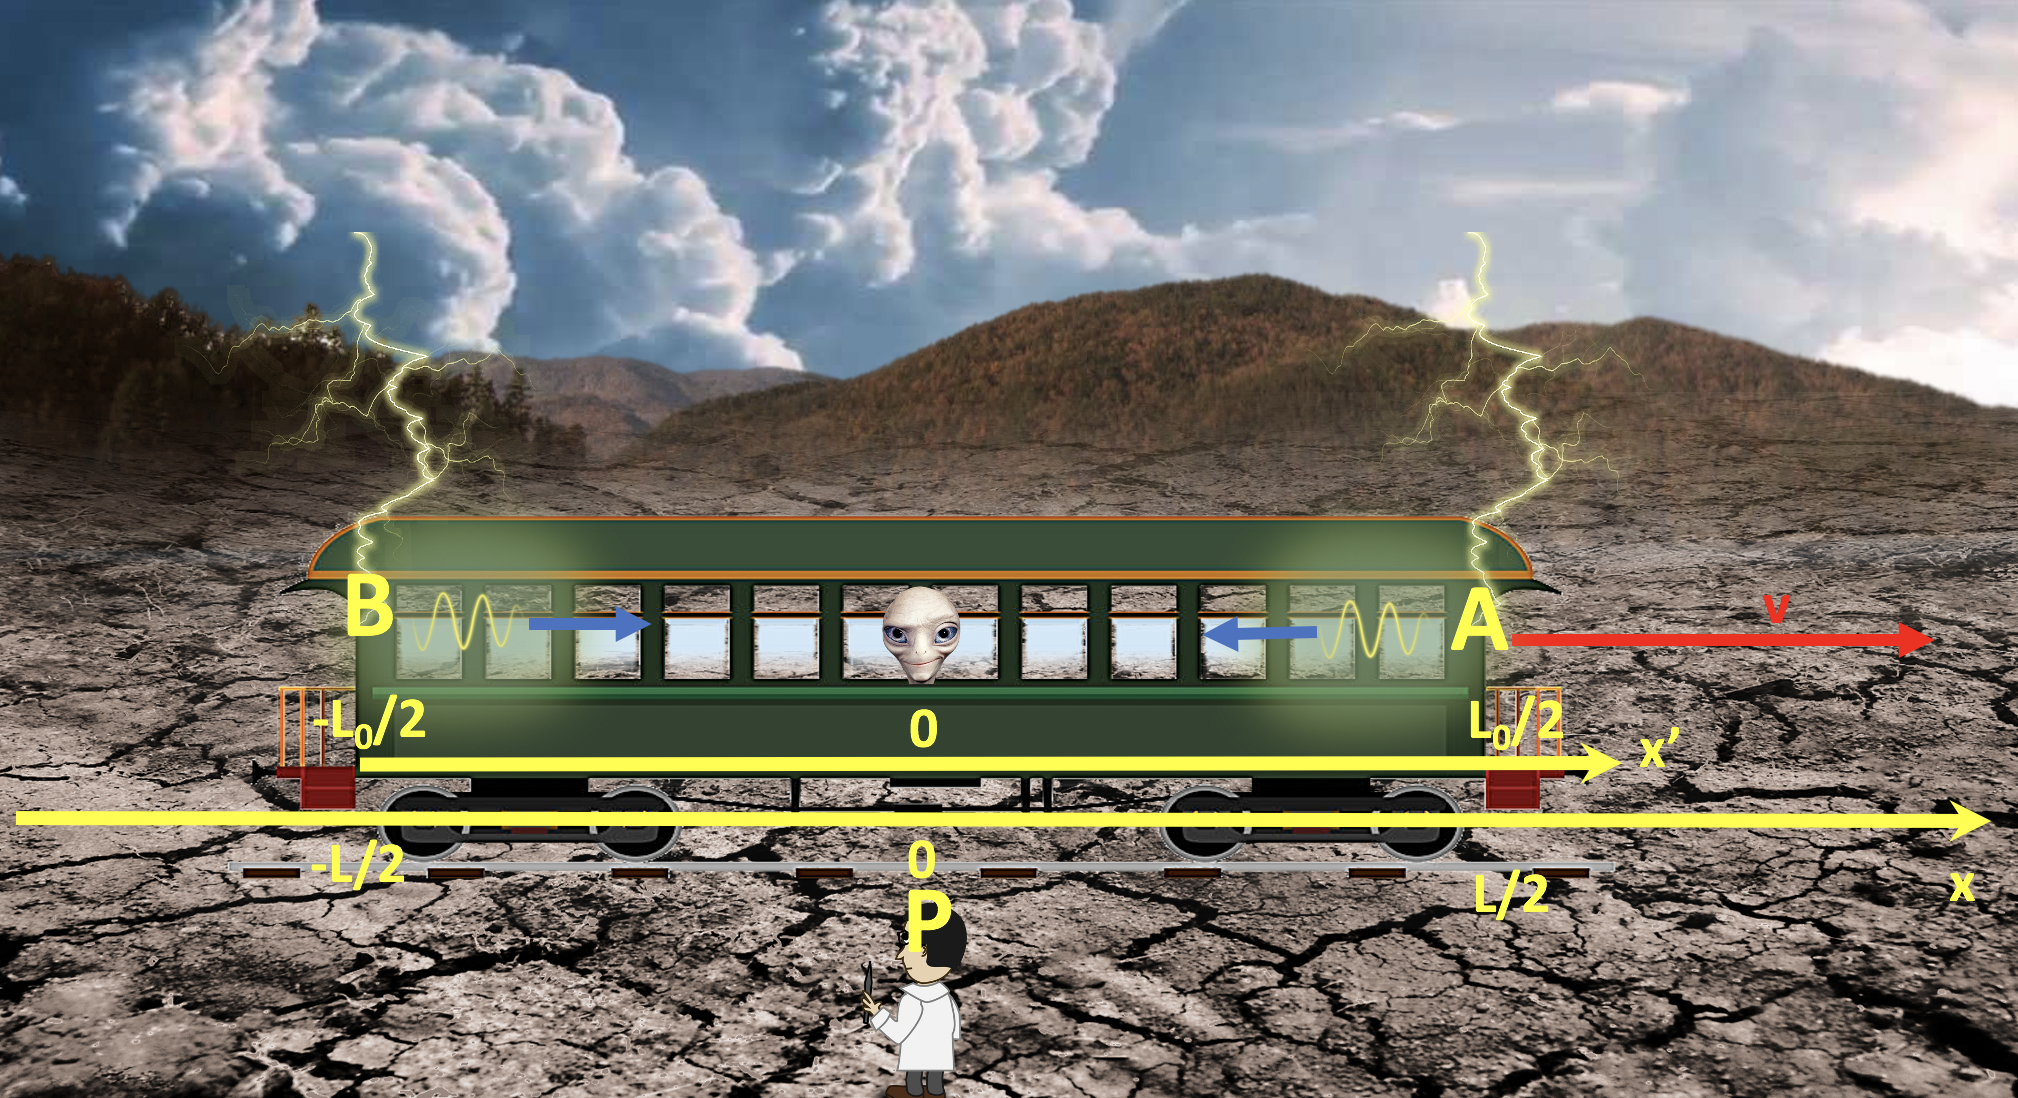
\includegraphics[scale=0.26]{media/tog7.png}}
{\footnotesize Det vi nå ønsker å finne er:
\begin{itemize}
\item hva er lengden $L_0$ av toget i togsystemet? (gitt at vi kjenner $L$ i labsystemet)
\item Ved hvilke tidspunkt $t_A'$ og $t_B'$ skjer de to lynnedslagene i togsystemet, altså målt på toget sin klokke? (vi vet jo nå når de skjer i labsystemet)
\end{itemize}
{\bf For å løse dette trenger vi, som alltid i denne type oppgave, å først skrive opp posisjon og tidspunkt til alle kjente hendelser, A, B og P i begge referansesystem.}}
}{SIDE 23/39/39}

\fullframe{tog5}{tog4}{tog6}{0}{\small
\centerline{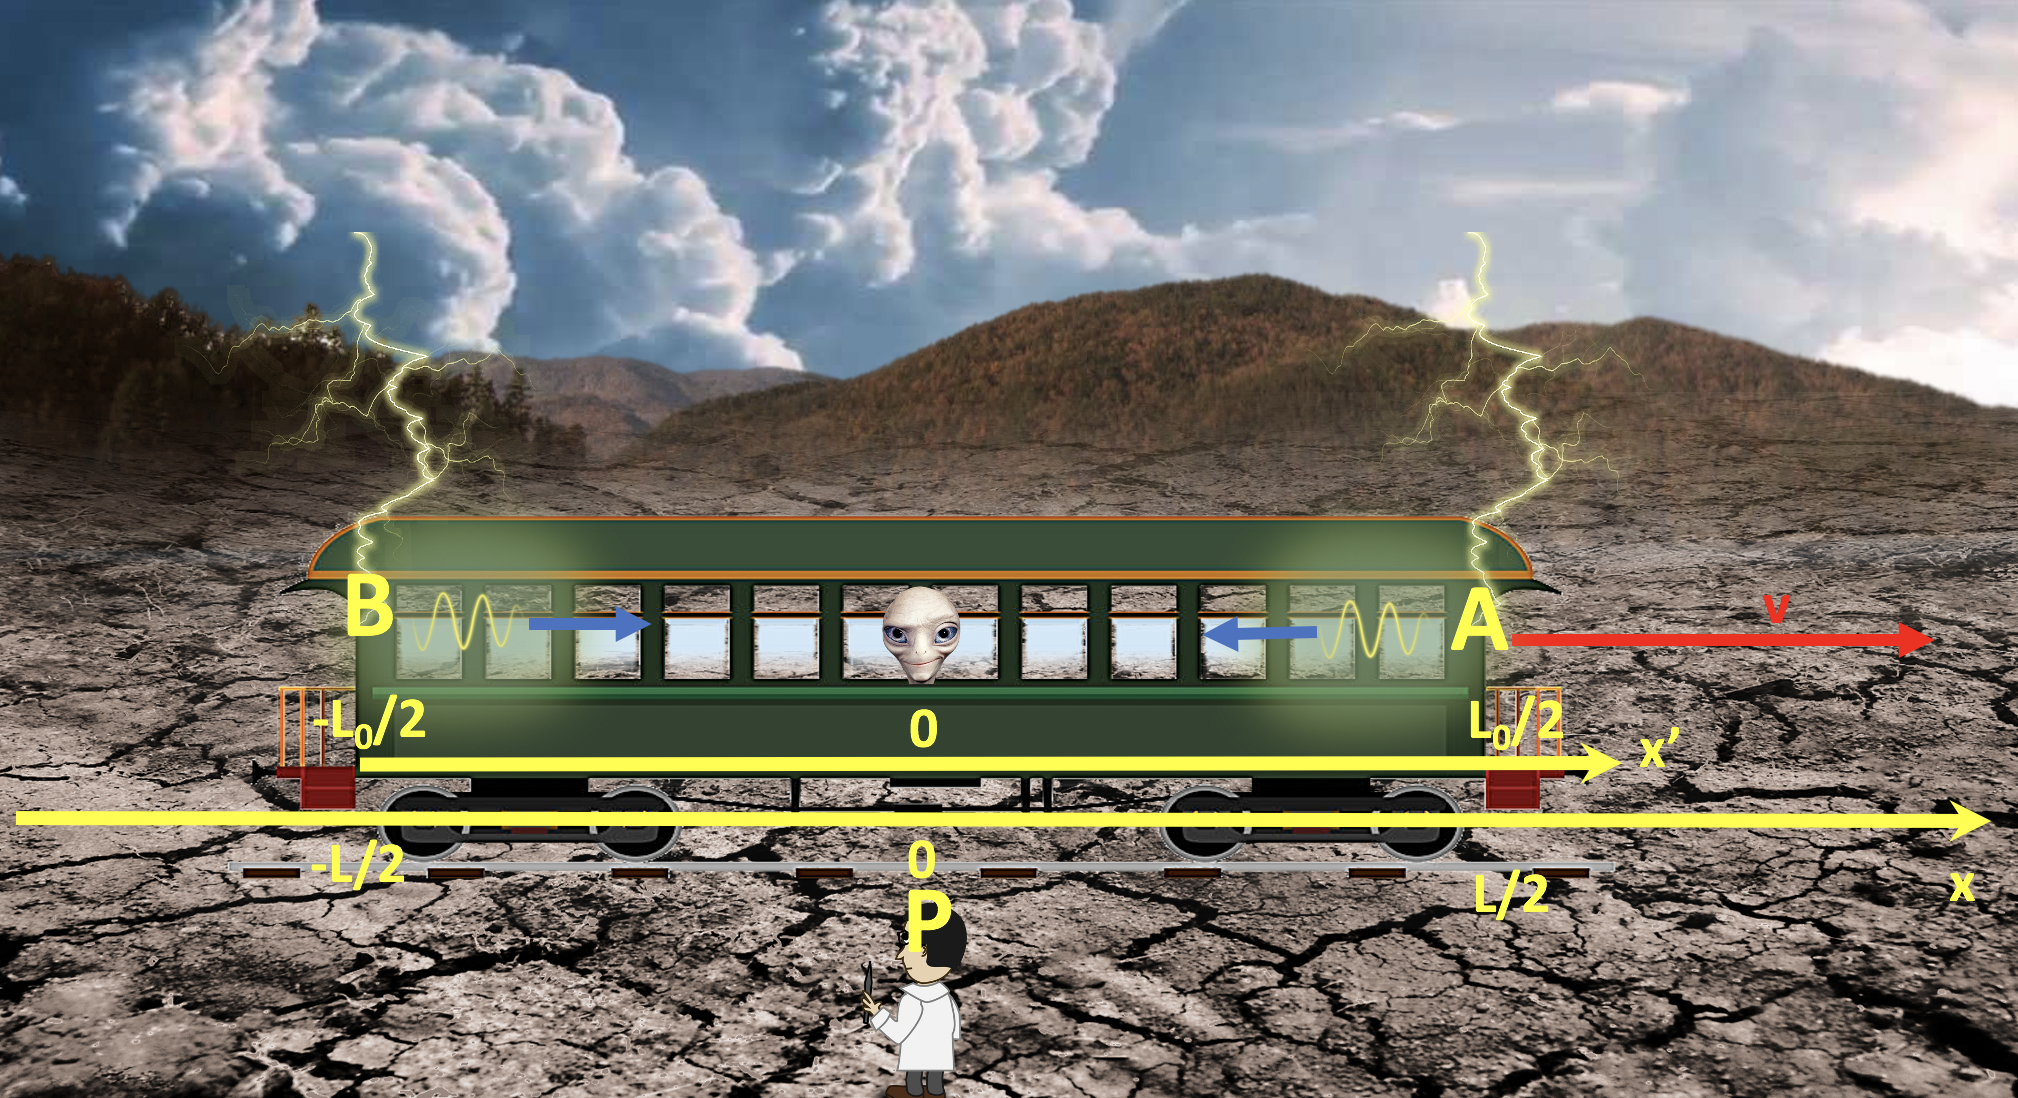
\includegraphics[scale=0.26]{media/tog7.png}}
Nå begynner jobben: Ta et stykke papir, lag en tabell med posisjoner og tidspunkter i merket og umerket system for alle tre hendelser. De skal uttrykkes kun ved den kjente størrelsen $L$ samt de ukjente størrelsene $L_0$, $t_A'$ og $t_B'$. Ikke gå videre før du har det.
}{SIDE 24/39/39}

\fullframe{tog6}{tog5}{tog7}{0}{
Fikk du:\\
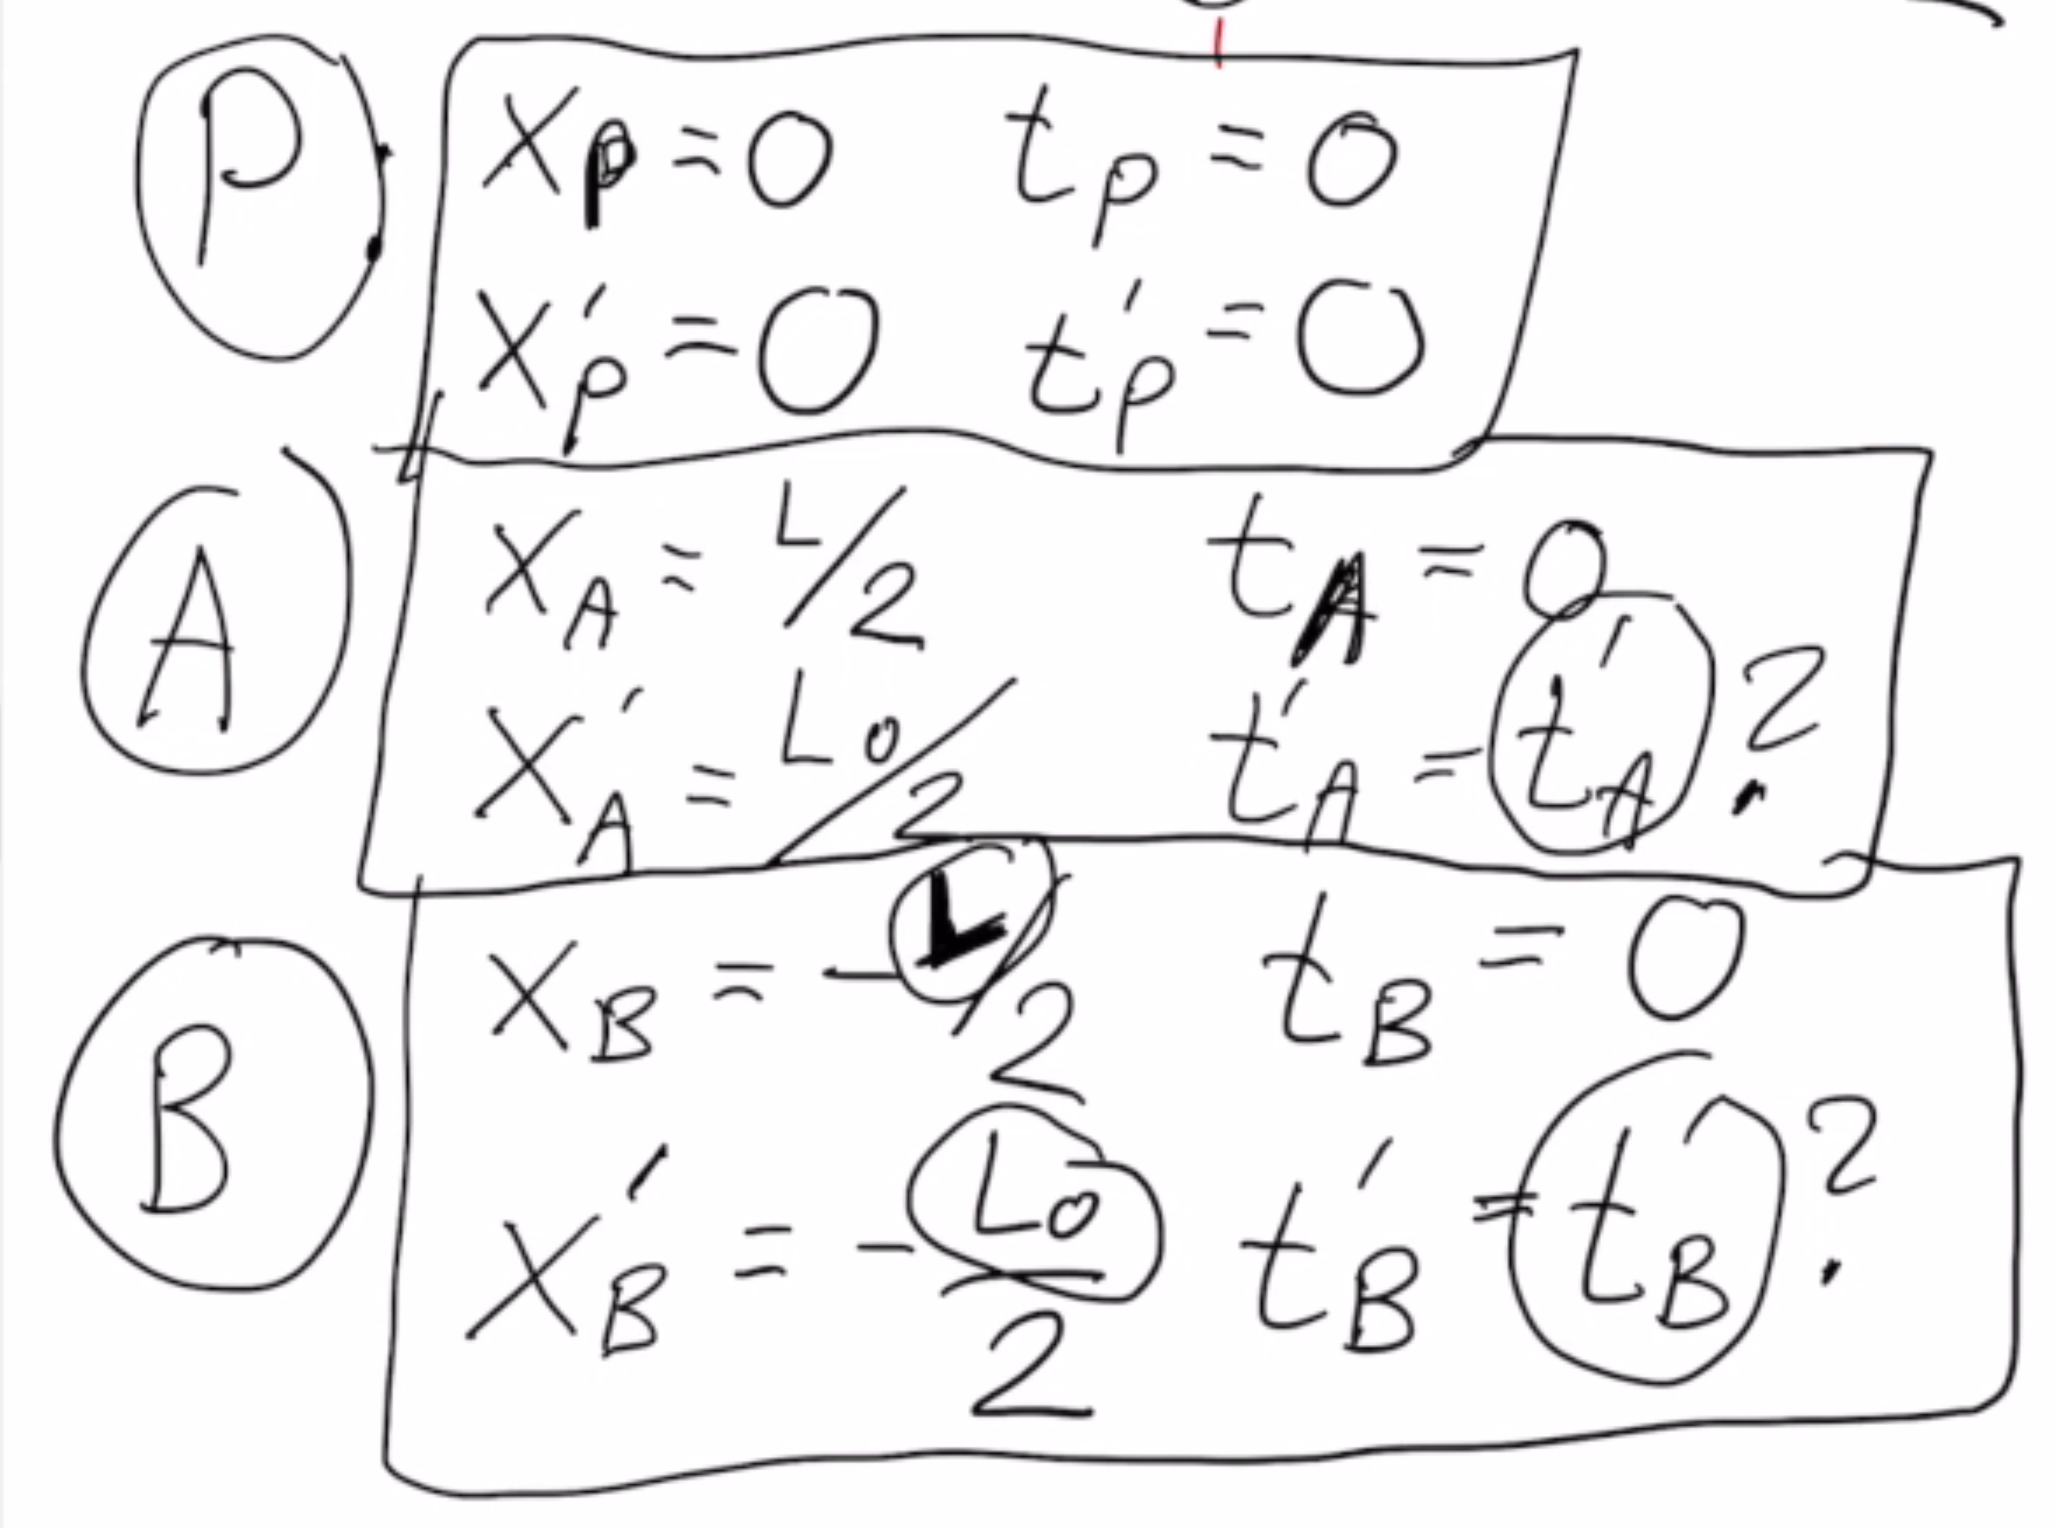
\includegraphics[scale=0.25]{media/abp_events.png}\\
Hvis ikke, eller hvis du er i tvil om noe, se hvordan vi kommer frem til dette i \href{https://www.uio.no/studier/emner/matnat/astro/AST2000/h20/undervisningsmateriell/interaktive-forelesningsnotater/2a/videoer/video2a_5.mp4}{denne videoen.}
}{SIDE 25/39/39}


\fullframe{tog7}{tog6}{tog8}{0}{\footnotesize
\centerline{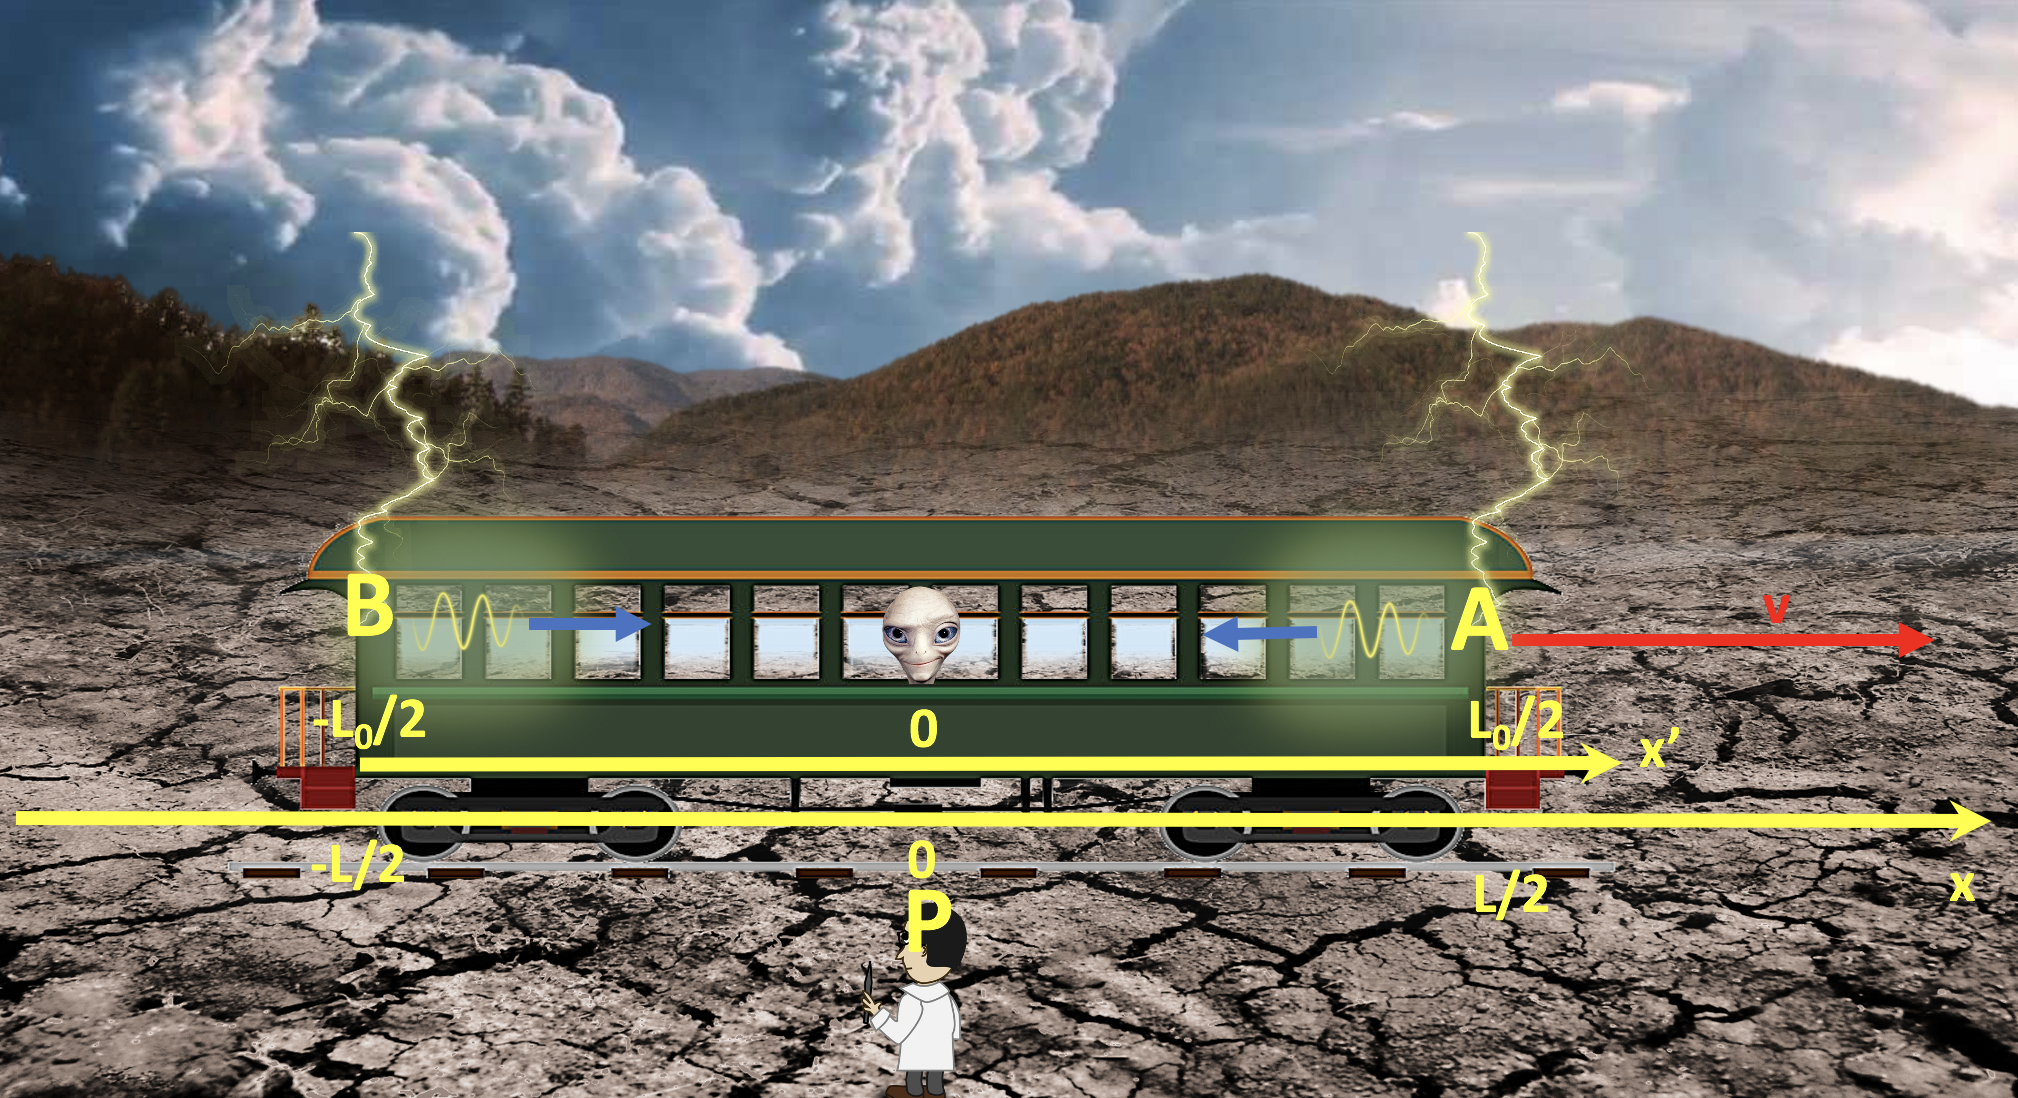
\includegraphics[scale=0.26]{media/tog7.png}}
{\tiny Vi har tre ukjent, $L_0$, $t_A'$ og $t_B'$, og trenger dermed tre likninger for å kunne finne disse. Vi vet nå at vi har en superviktig informasjon: tidromsintervallet er den samme i alle referansesystemer. Det vil si at $\Delta s$ er den samme i merket og umerket system for alle kombinasjoner av avstander mellom eventer. Ta nå utgangspunkt i avstanden mellom eventene A og B, sett opp invarians av tidromsintervallet og se om du kan komme frem til at:
\[
L^2=L_0^2-(t_A'-t_B')^2
\]
Som er en av de tre likningene vi trenger. Fikk du det ikke til, ta en titt på \href{https://www.uio.no/studier/emner/matnat/astro/AST2000/h20/undervisningsmateriell/interaktive-forelesningsnotater/2a/videoer/video2a_6.mp4}{denne videoen}.}
}{SIDE 26/39/39}

\fullframe{tog8}{tog7}{tog9}{0}{\small
\centerline{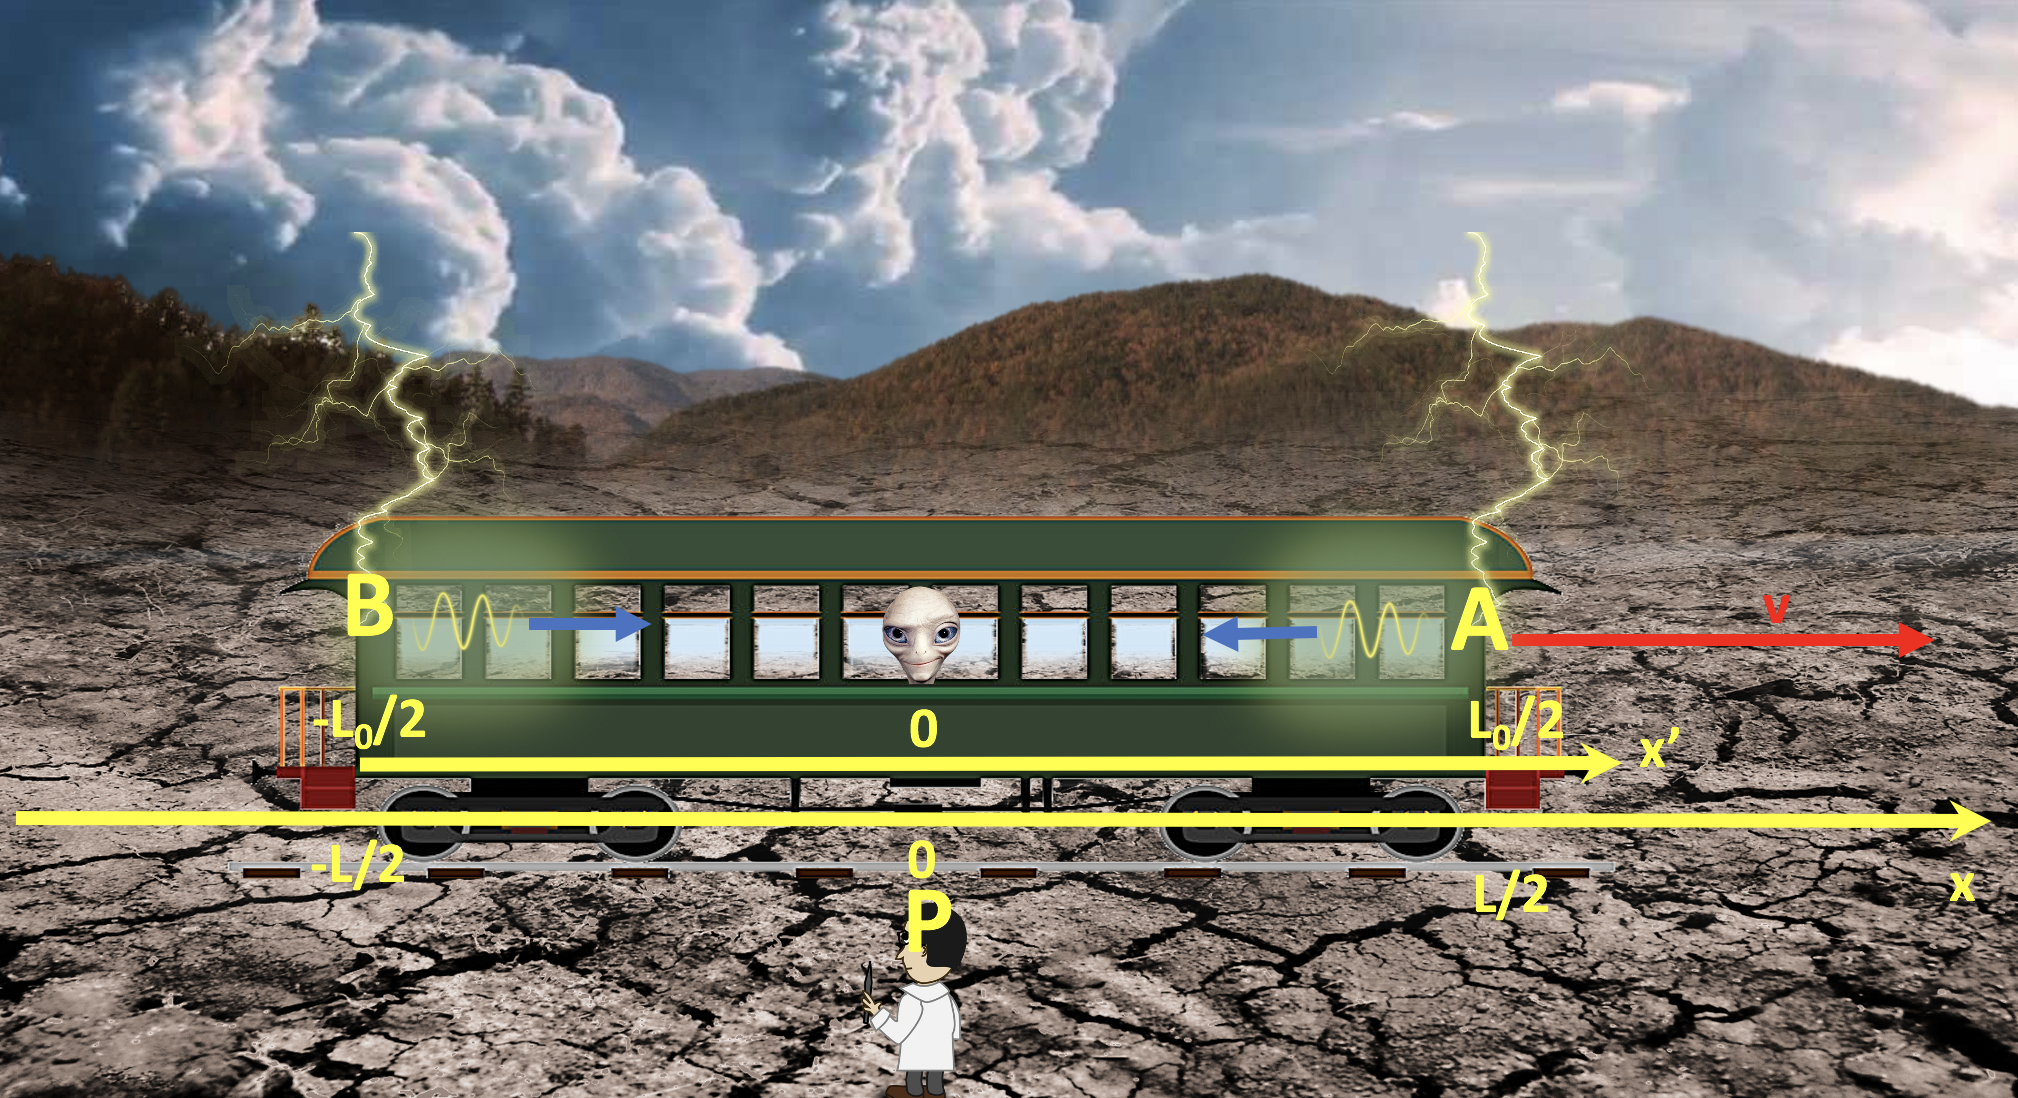
\includegraphics[scale=0.26]{media/tog7.png}}
Vi finner en likning til ved å bruke avstanden mellom eventene A og P, sett opp invarians av tidromsintervallet og se om du kan komme frem til at:
\[
(L/2)^2=(L_0/2)^2-(t_A')^2
\]
Som er den andre av de tre likningene vi trenger. Fikk du det ikke til, ta en titt på \href{https://www.uio.no/studier/emner/matnat/astro/AST2000/h20/undervisningsmateriell/interaktive-forelesningsnotater/2a/videoer/video2a_7.mp4}{denne videoen}.
}{SIDE 27/39/39}


\fullframe{tog9}{tog8}{tog10}{0}{\small
\centerline{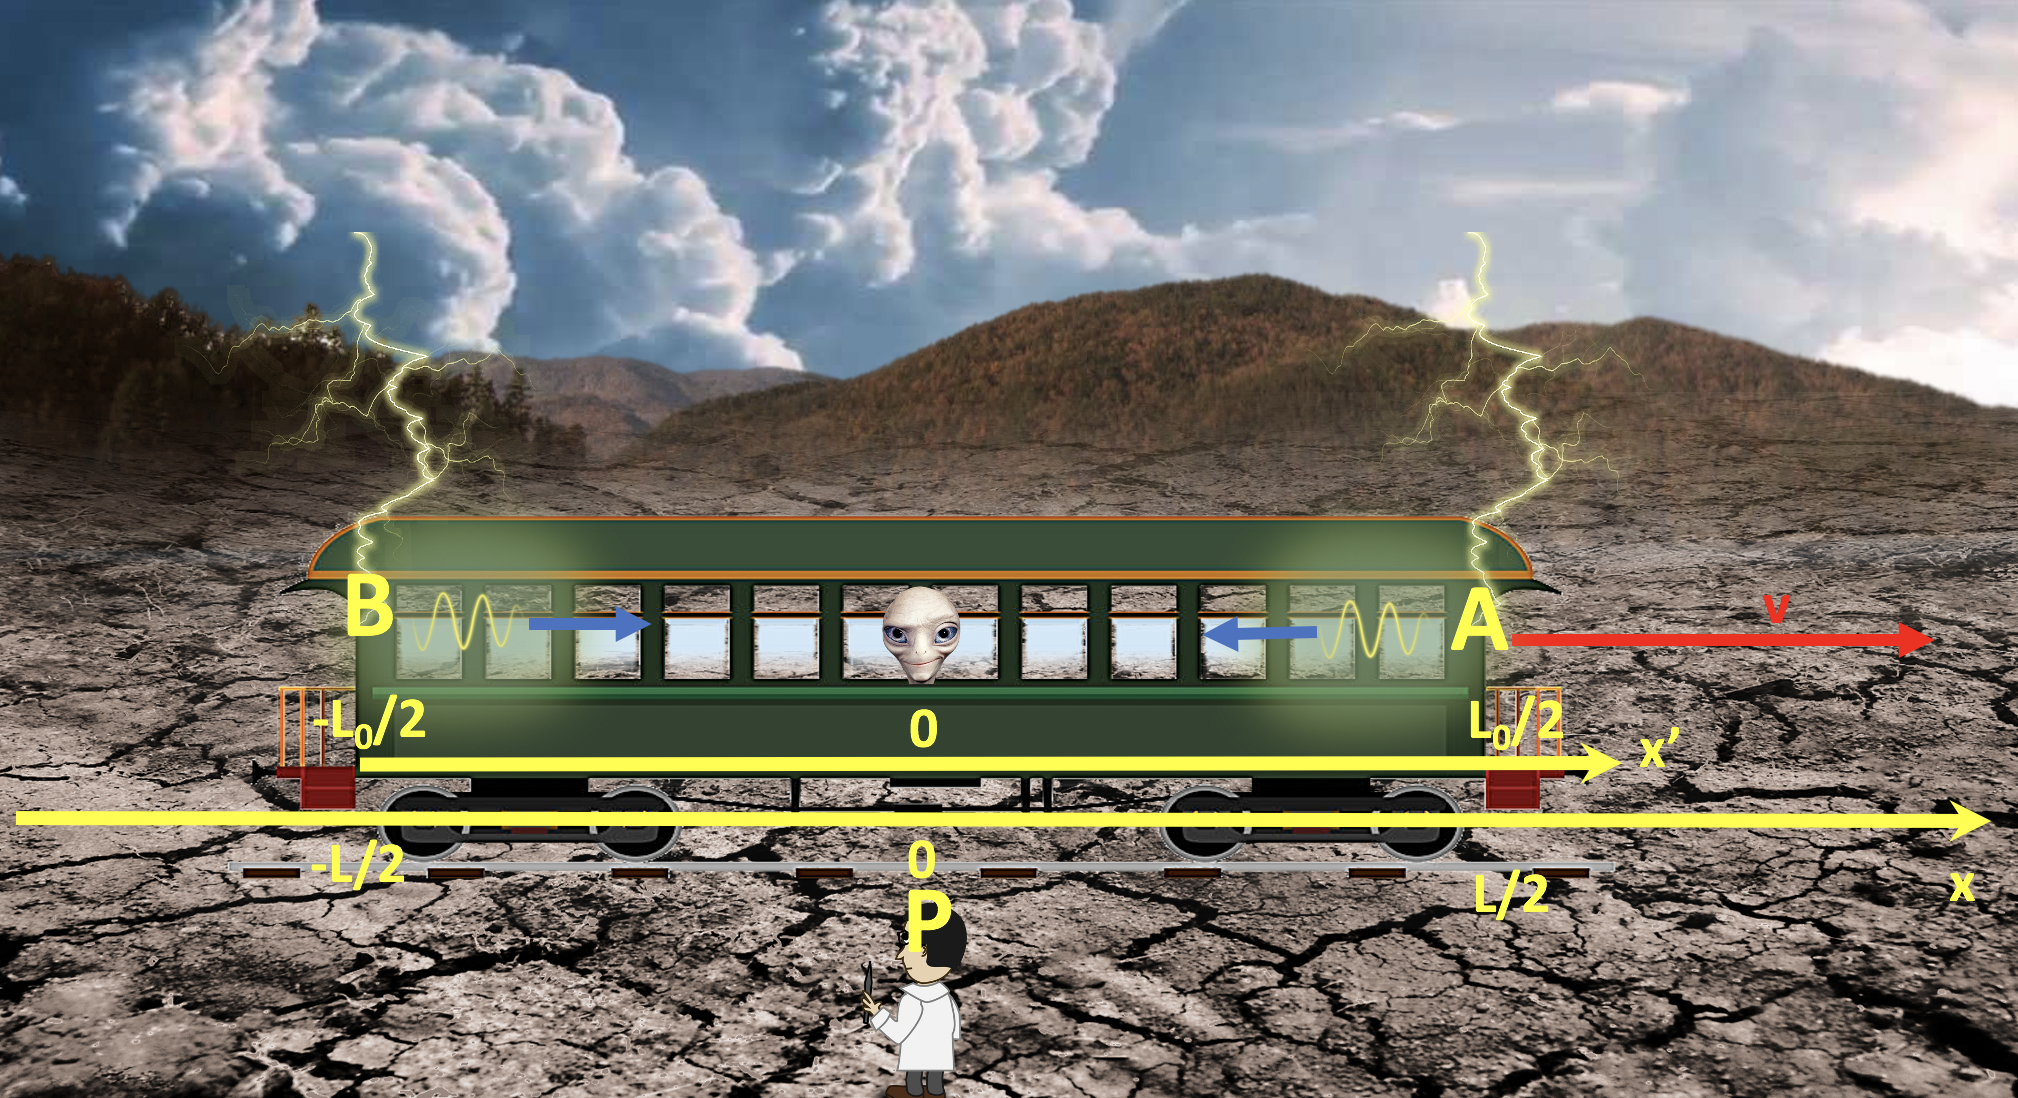
\includegraphics[scale=0.26]{media/tog7.png}}
Nå er det fristende å bruke avstanden mellom B og P for å finne den 3. likningen. Dessverre, siden vi allerede har brukt alle disse eventene, så gir ikke dette oss noen ny informasjon. Dette er en typisk situasjon: da må vi finne oss et event til, {\bf men} vi må passe på at dette eventet ikke gir oss en ekstra ukjent, for da er vi like langt. Kan du tenke deg et slikt event her?
}{SIDE 28/39/39}

\fullframe{tog10}{tog9}{tog11}{0}{\small
\centerline{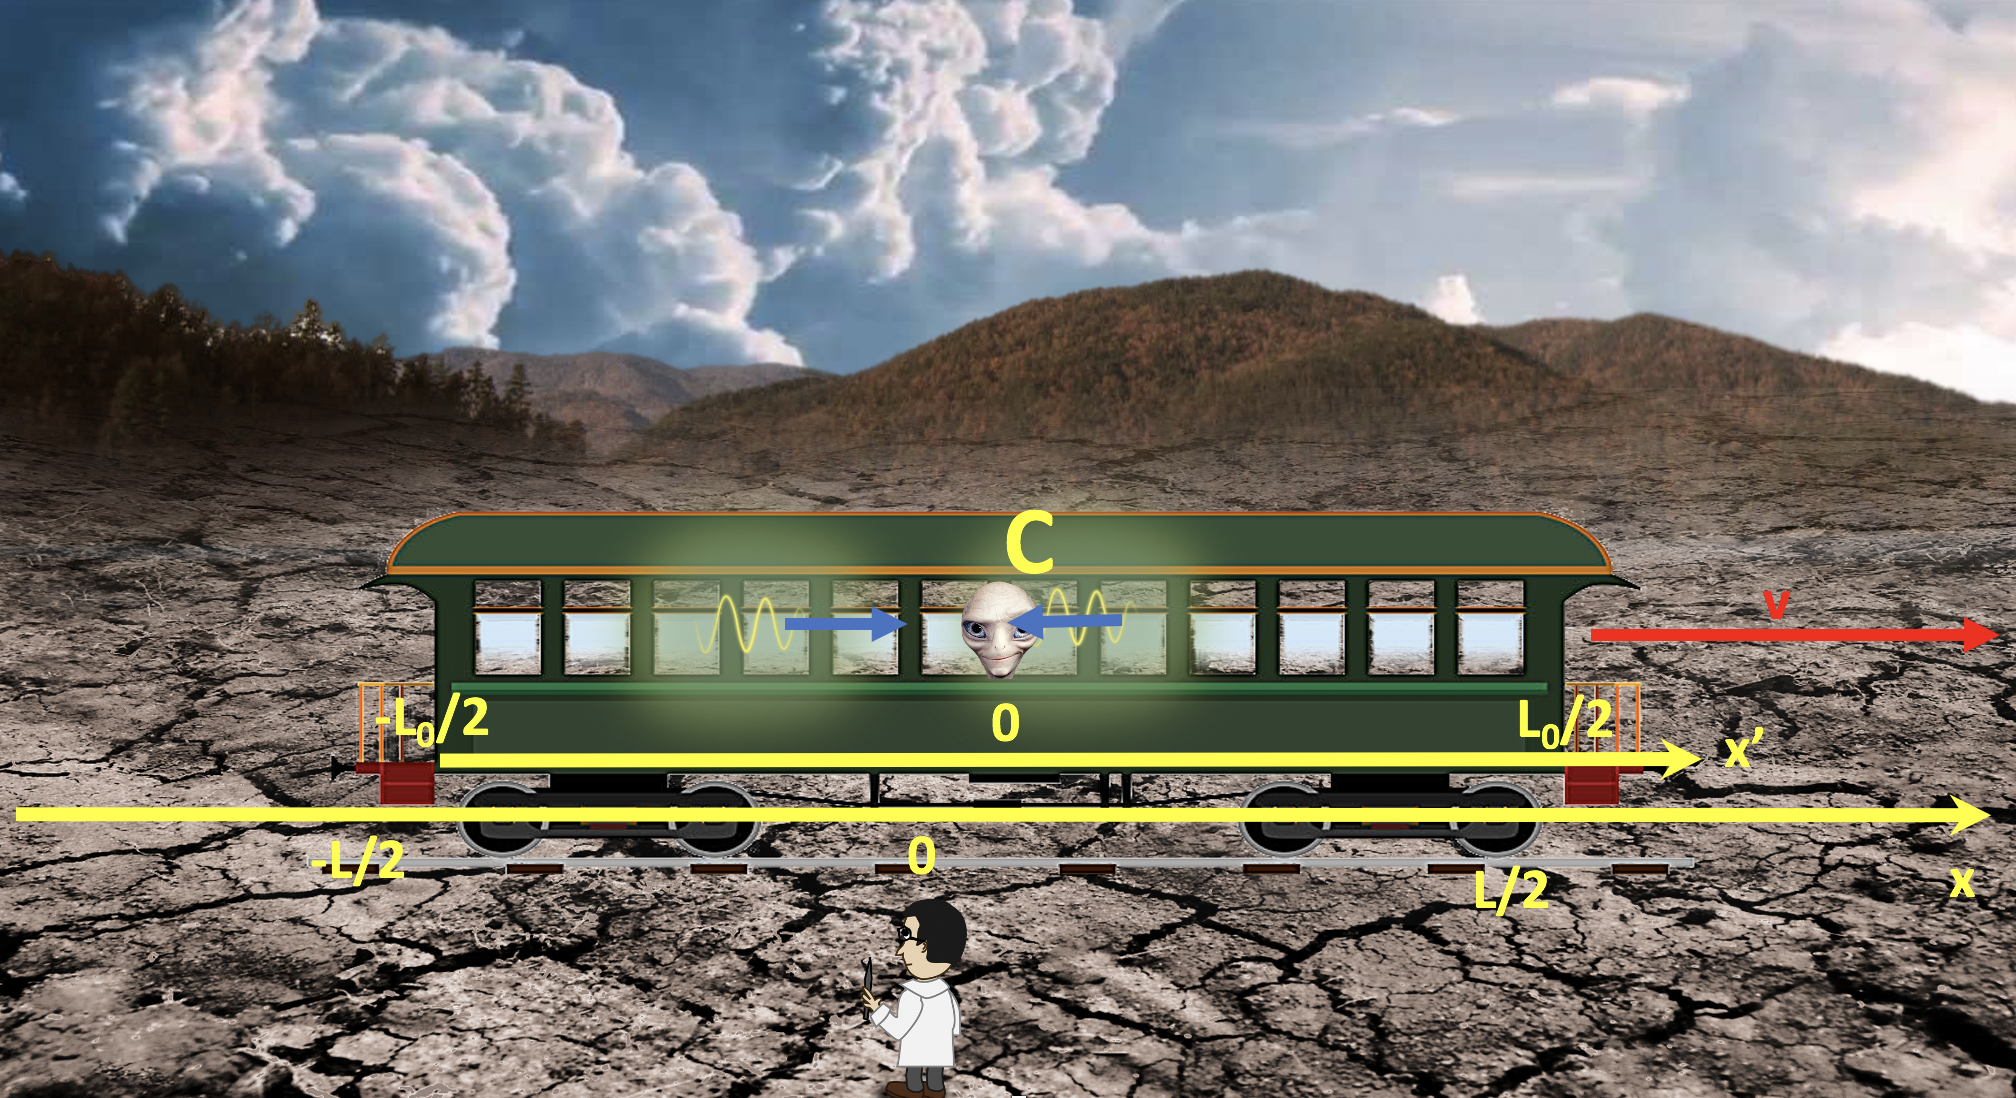
\includegraphics[scale=0.26]{media/tog8.png}}
{\footnotesize Husker du event C og D fra første forelesning? Eventene når passasjer P ser de to lysglimtene? Kunne vi bruke en eller begge av disse? Det kunne jo til og med være interessant å vite hvilke tidspunkt disse skjer på. {\bf Det er jo f.eks. interessant å vite om passasjer P ser lysglimtene fra lynene før eller etter at professor O hilser på passasjer P!}. Men hva er posisjonene og tidspunktene til event C og D? Tidspunktene i labsystemet som vi fant i forelesning 1 er vel enda riktige? Og tankegangen der for å finne disse tidspunktene i togsystemet kan vi vel også bruke?}
}{SIDE 29/39/39}


\fullframe{tog11}{tog10}{tog12}{0}{\small
\centerline{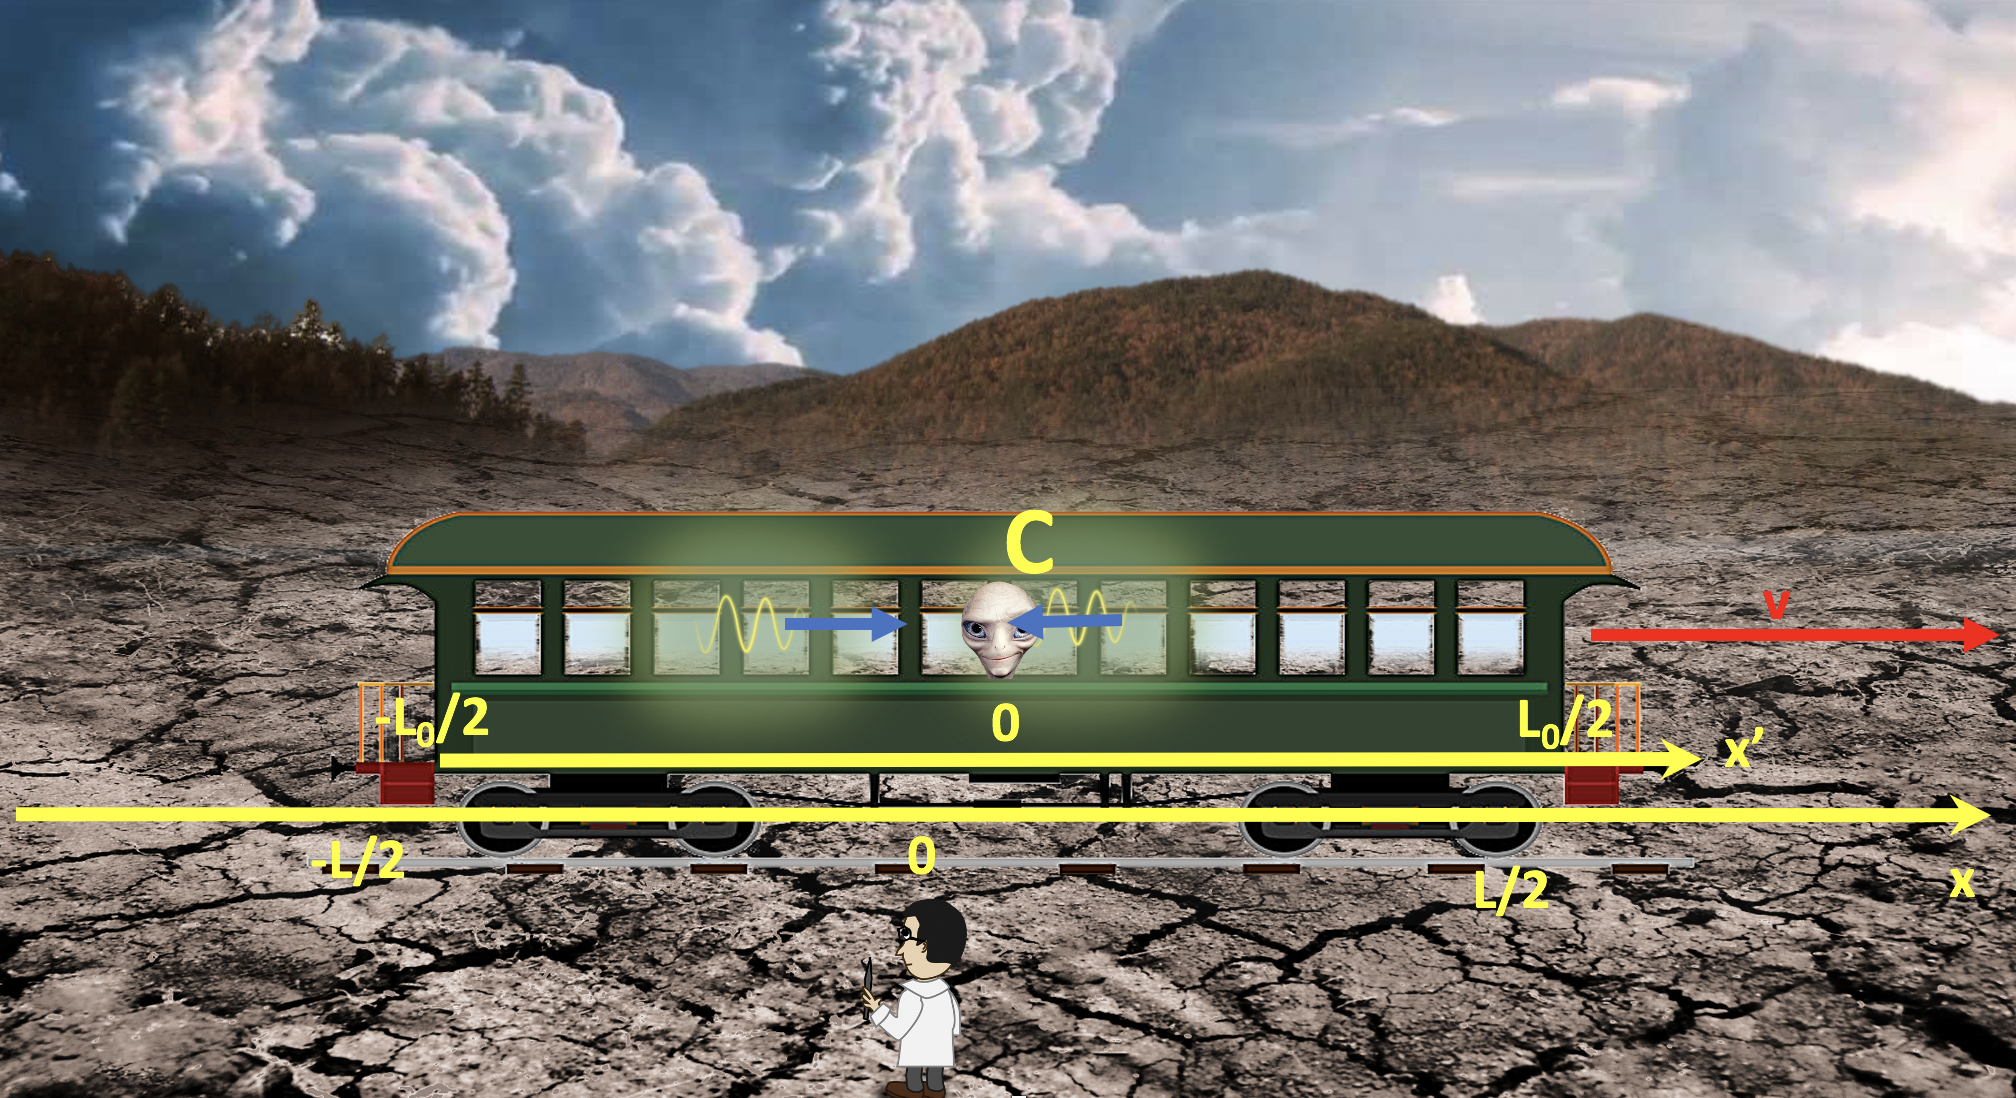
\includegraphics[scale=0.26]{media/tog8.png}}
Tenk gjennom hvordan du kan finne posisjoner og tidspunkter til event C og D i begge referansesystemer og skriv disse opp i en tabell. Bruk gjerne tenkemåten fra forelesning 1. Ikke gå videre før du har fylt ut tabellen.
}{SIDE 30/39/39}

\fullframe{tog12}{tog11}{tog13}{0}{
Fikk du:\\
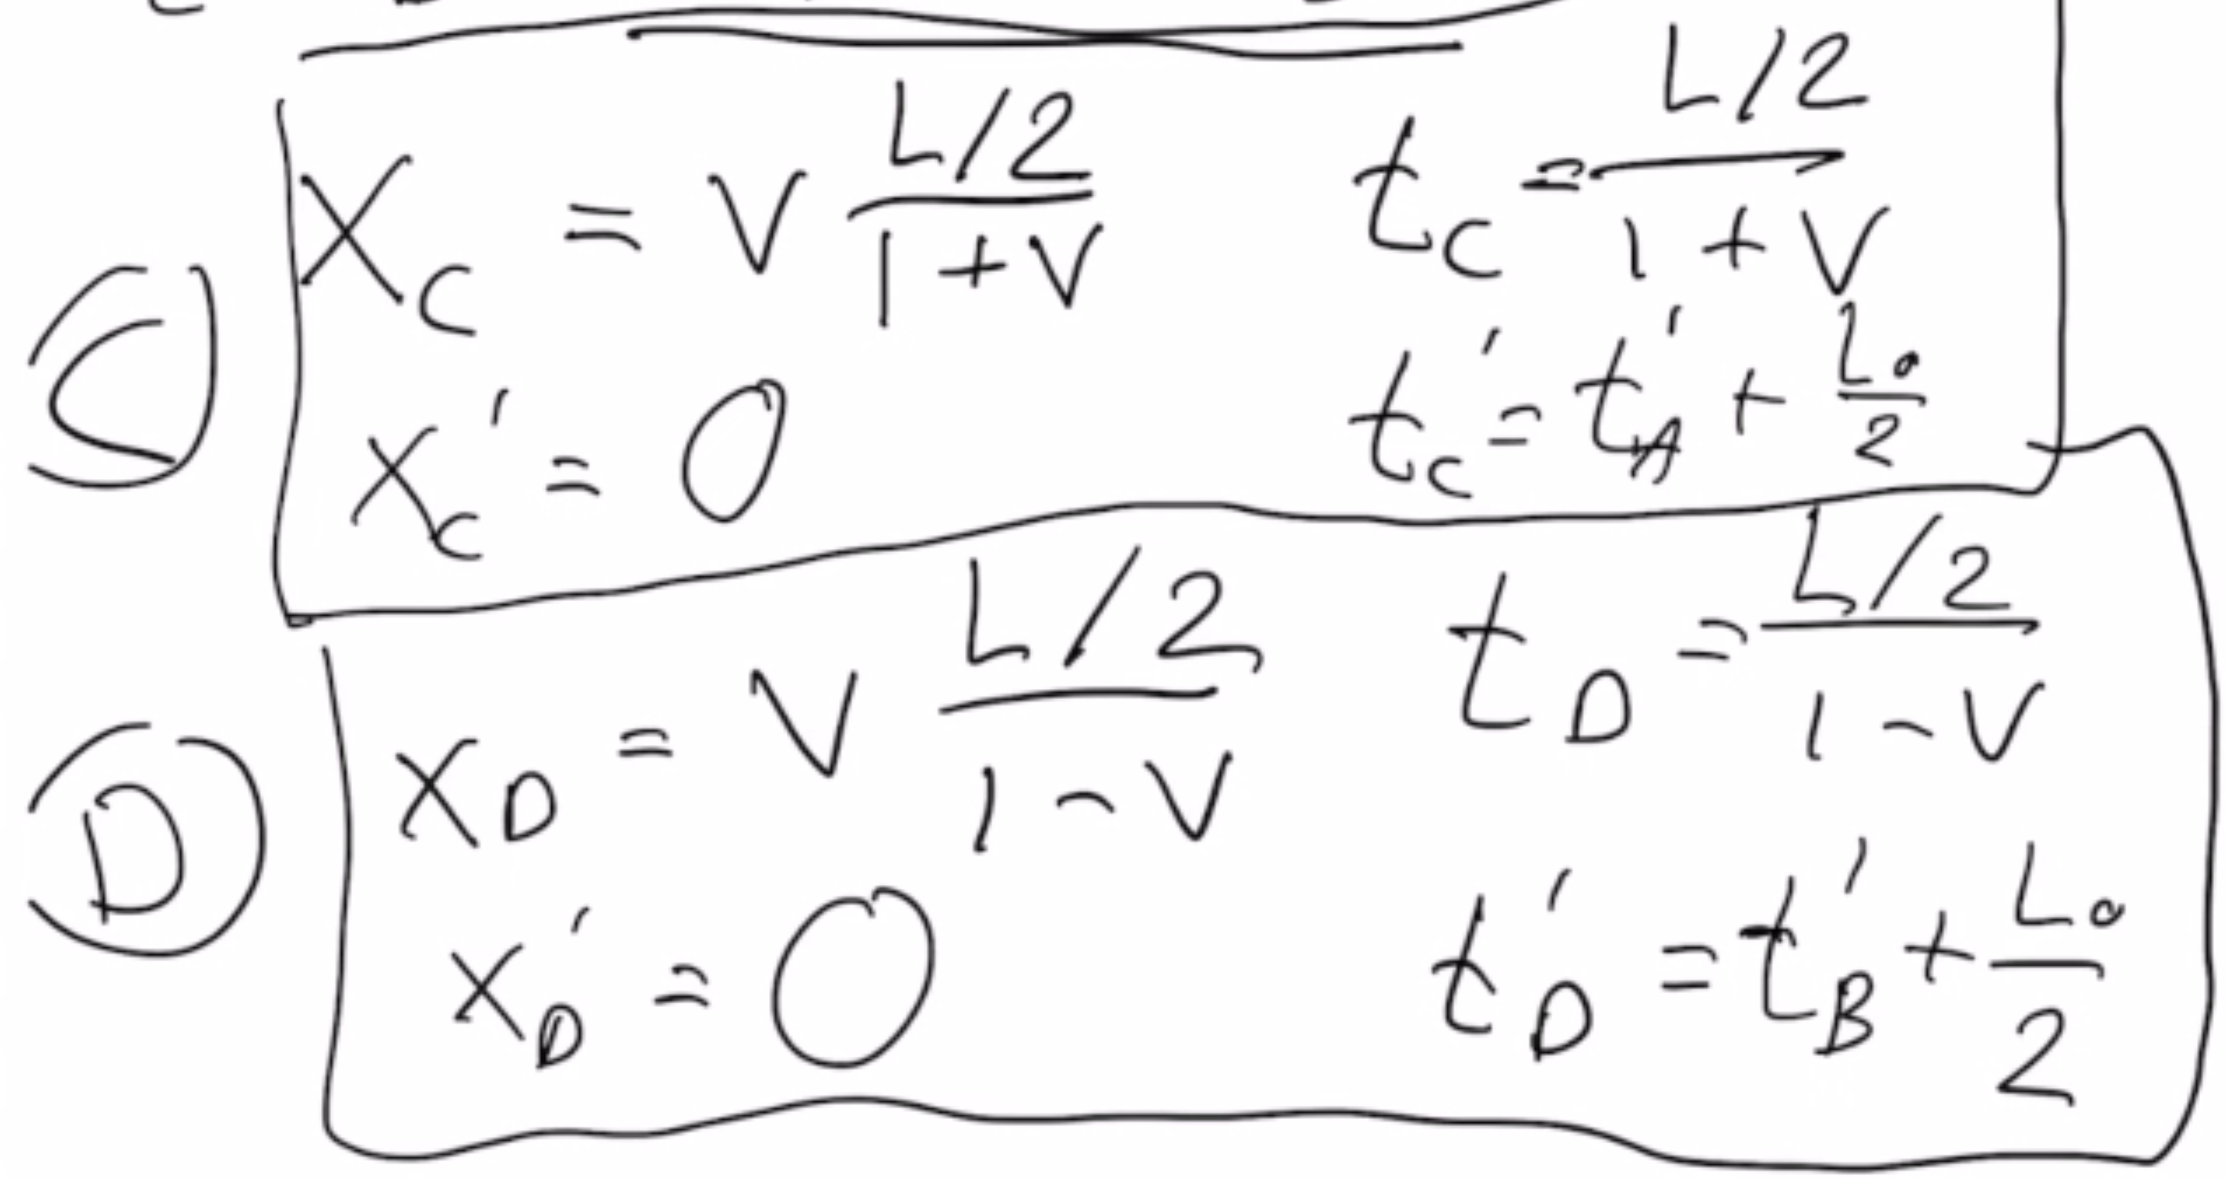
\includegraphics[scale=0.25]{media/cd_events.png}\\
Hvis ikke, eller hvis du er i tvil om noe, se hvordan vi kommer frem til dette i \href{https://www.uio.no/studier/emner/matnat/astro/AST2000/h20/undervisningsmateriell/interaktive-forelesningsnotater/2a/videoer/video2a_8.mp4}{denne videoen.}
}{SIDE 31/39/39}

\fullframe{tog13}{tog12}{pause2}{0}{\small
\centerline{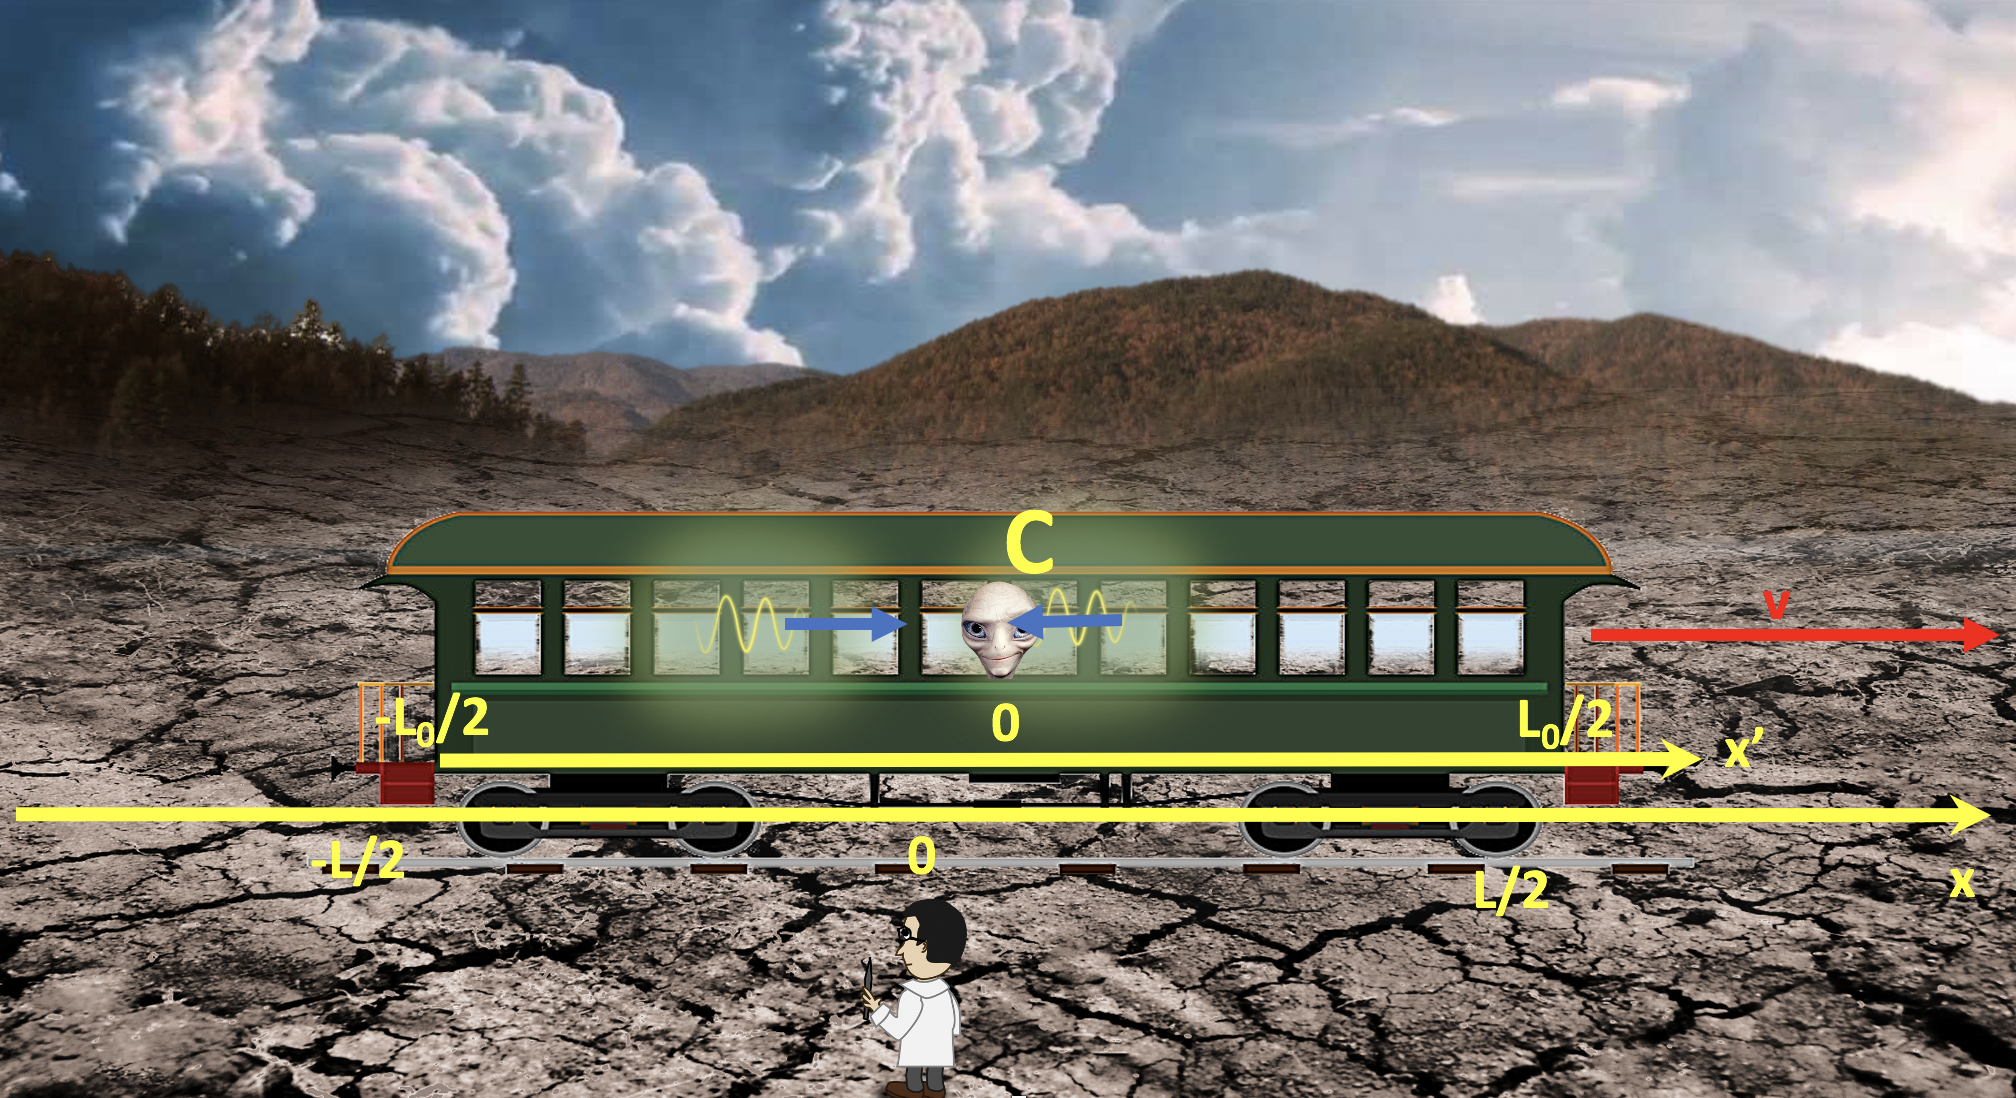
\includegraphics[scale=0.26]{media/tog8.png}}
La oss nå finne den 3. likningen vår ved å bruke avstanden mellom eventene C og P (P er et veldig praktisk event å bruke siden alt er 0 og vi får finere likninger), sett opp invarians av tidromsintervallet og se om du kan komme frem til at:
\[
\frac{(L/2)^2}{(1+v)^2}(1-v^2)=(t_A'+L_0/2)^2
\]
Som er den siste av de tre likningene vi trenger. Fikk du det ikke til, ta en titt på \href{https://www.uio.no/studier/emner/matnat/astro/AST2000/h20/undervisningsmateriell/interaktive-forelesningsnotater/2a/videoer/video2a_9.mp4}{denne videoen}.
}{SIDE 32/39/39}

{
\setbeamercolor{background canvas}{bg=cyan}
\begin{frame}
\label{pause2}
\hyperlink{tog13}{\pagebutton{\small Forrige side}}
{\Large
\centerline{Kakaopause}
\centerline{
\includegraphics[scale=4]{media/drink-coffee.png}}\\
Kulda setter inn, og litt kakao må man kunne kose seg med oppi all denne abstrakte tenkingen og regningen. For å prøve å se den 4 dimensjonen anbefales det å bruke denne pausen til å stå på hodet (jeg mener det, vel, ihvertfall for å få litt blod til hodet). Bruk veggen til hjelp. Og en tur i frisk luft er absolutt påkrevet før du går videre. Ikke finn på å fortsette før hodet er klart igjen!
}\\
\vspace*{0.5cm}
\hyperlink{tog14}{\pagebutton{Ok, ok, tankene er klarnet...}}
\end{frame}
}


\fullframenotxt{tog14}{tog13}{tog15}{0}{\footnotesize
Vi har altså fått disse 3 likningene med 3 ukjente:
\begin{align}
\label{eq:AB}L^2&=L_0^2-(t_A'-t_B')^2\\
\label{eq:AP}(L/2)^2&=(L_0/2)^2-(t_A')^2\\
\label{eq:CP}\frac{(L/2)^2}{(1+v)^2}(1-v^2)&=(t_A'+L_0/2)^2
\end{align}
Sett inn for L i likning (3) fra likning (2). Da skulle du få to mulige løsninger for $t_A'$. Hvilke?\hyperlink{tog14_b}{\pagebutton{\small Wow, det blir litt lang regning...}}
\textcolor{white}{
Fikk du:
\begin{align*}
t_A'&=-L_0/2\\
t_A'&=-vL_0/2
\end{align*}
??? Men kun en løsning kan være riktig. Kan du se at det er noe veldig ufysisk med en av disse løsningene? (hint: hva betyr $t_A'$? Hva blir $t_C'$ gitt disse løsningene? Og hva er tolkningen av det?){\small Jeg har tenkt litt!}\\
Løsningen $t_A=-L_0/2$ er ufysisk. Hvis du er usikker, både på hvordan vi kom frem til disse to løsningene og hvorfor den ene løsningen er ufysisk, se på {denne videoen}.{\bf (Merk at videoen har lang og stygg regning, hvis du ikke er interessert i detaljer, spol frem til tolkning av det ufysiske resultatet)}}
}{SIDE 33/39/39}

\fullframenotxt{tog14_b}{tog13}{tog15}{0}{\footnotesize
Vi har altså fått disse 3 likningene med 3 ukjente:
\setcounter{equation}{0}
\begin{align}
L^2&=L_0^2-(t_A'-t_B')^2\\
(L/2)^2&=(L_0/2)^2-(t_A')^2\\
\frac{(L/2)^2}{(1+v)^2}(1-v^2)&=(t_A'+L_0/2)^2
\end{align}
Sett inn for L i likning (3) fra likning (2). Da skulle du få to mulige løsninger for $t_A'$. Hvilke?\pagebutton{\small Wow, det blir litt lang regning...}
Fikk du:
\begin{align*}
t_A'&=-L_0/2\\
t_A'&=-vL_0/2
\end{align*}
??? Men kun en løsning kan være riktig. Kan du se at det er noe veldig ufysisk med en av disse løsningene? (hint: hva betyr $t_A'$? Hva blir $t_C'$ gitt disse løsningene? Og hva er tolkningen av det?)\hyperlink{tog14_c}{\pagebutton{\small Jeg har tenkt litt!}}
\textcolor{white}{
Løsningen $t_A=-L_0/2$ er ufysisk. Hvis du er usikker, både på hvordan vi kom frem til disse to løsningene og hvorfor den ene løsningen er ufysisk, se på {denne videoen}.{\bf (Merk at videoen har lang og stygg regning, hvis du ikke er interessert i detaljer, spol frem til tolkning av det ufysiske resultatet)}}
}{SIDE 33/39/39}

\fullframe{tog14_c}{tog13}{tog15}{0}{\footnotesize
Vi har altså fått disse 3 likningene med 3 ukjente:
\setcounter{equation}{0}
\begin{align}
L^2&=L_0^2-(t_A'-t_B')^2\\
(L/2)^2&=(L_0/2)^2-(t_A')^2\\
\frac{(L/2)^2}{(1+v)^2}(1-v^2)&=(t_A'+L_0/2)^2
\end{align}
Sett inn for L i likning (3) fra likning (2). Da skulle du få to mulige løsninger for $t_A'$. Hvilke?\pagebutton{\small Wow, det blir litt lang regning...}
Fikk du:
\begin{align*}
t_A'&=-L_0/2\\
t_A'&=-vL_0/2
\end{align*}
??? Men kun en løsning kan være riktig. Kan du se at det er noe veldig ufysisk med en av disse løsningene? (hint: hva betyr $t_A'$? Hva blir $t_C'$ gitt disse løsningene? Og hva er tolkningen av det?)\pagebutton{\small Jeg har tenkt litt!}
Løsningen $t_A=-L_0/2$ er ufysisk. Hvis du er usikker, både på hvordan vi kom frem til disse to løsningene og hvorfor den ene løsningen er ufysisk, se på \href{https://www.uio.no/studier/emner/matnat/astro/AST2000/h20/undervisningsmateriell/interaktive-forelesningsnotater/2a/videoer/video2a_10.mp4}{denne videoen}.{\bf (Merk at videoen har lang og stygg regning, hvis du ikke er interessert i detaljer, spol frem til tolkning av det ufysiske resultatet)}
}{SIDE 33/39/39}


\fullframe{tog15}{tog14}{tog15x}{1}{\small
Vi har altså
\setcounter{equation}{0}
\begin{align}
L^2&=L_0^2-(t_A'-t_B')^2\label{eq:AB}\\
(L/2)^2&=(L_0/2)^2-(t_A')^2\label{eq:AP}\\
\frac{(L/2)^2}{(1+v)^2}(1-v^2)&=(t_A'+L_0/2)^2\label{eq:CP}
\end{align}
og vet nå at $t_A'=-vL_0/2$. Kan du se hvordan vi kan gå videre og finne et uttrykk for $t_B'$ og en sammenheng mellom $L$ og $L_0$? I \href{https://www.uio.no/studier/emner/matnat/astro/AST2000/h20/undervisningsmateriell/interaktive-forelesningsnotater/2a/videoer/video2a_11.mp4}{denne videoen} ser du hvordan det kan gjøres. (Merk at det igjen er litt stygg regning i starten, spol frem hvis du ikke er interessert). Du får også en tolkning av $L_0$ som {\bf hvilelengden} eller {\bf egenlengden} av toget (på engelsk: proper length). Dette er et begrep som du må kjenne til og forstå.
}{SIDE 34/39/39}

\fullframe{tog15x}{tog15}{tog16}{0}{
Vi fikk altså som resultat at:
\begin{align*}
t_A'&=-vL_0/2\\
t_B'&=vL_0/2\\
L&=L_0\sqrt{1-v^2}=\frac{L_0}{\gamma}
\end{align*}
Vi ser altså at lynet A i togsystemet slo ned {\bf før} $t'=0$ mens B slo ned {\bf etter} $t'=0$, og symmetrisk om $t'=0$. Vi ser sammenhengen mellom lengden $L$ av et objekt i bevegelse og lengden $L_0$ av det samme objektet i hvilesystemet til dette objektet, altså systemet der dette objektet er i ro. Vi har også introdusert Lorentzfaktoren her:
\[
\gamma=\frac{1}{\sqrt{1-v^2}}
\]
}{SIDE 35/39/39}



\fullframe{tog16}{tog15x}{tog17}{0}{\small
Nå kan vi også finne $t_C'$ og $t_D'$ og tolke disse. Det gjør vi \href{https://www.uio.no/studier/emner/matnat/astro/AST2000/h20/undervisningsmateriell/interaktive-forelesningsnotater/2a/videoer/video2a_12.mp4}{i denne videoen her} samtidig som vi der også finner en sammenheng mellom et tidsintervall i to referansesystemer. Vi ser spesifikt på sammenhengen mellom intervallet $\Delta t_{CD}$ i labsystemet og $\Delta t_{CD}'$ i togsystemet. Altså hvor lang tid det tok fra lysglimtet fra A traff P til lysglimtet fra B traff P, målt i det ene og det andre referansesystemet. Et tidsintervall mellom to eventer i det referansesystemet der disse to eventene skjer på samme koordinat, slik som C og D i togsystemet i dette tilfellet, kalles {\bf egentiden} (engelsk: proper time). Det var denne som vi i forrige eksempel (eksmpel 1) fant til å være like tidromsintervallet.
}{SIDE 36/39/39}

\fullframe{tog17}{tog16}{tog18}{0}{\small
I \href{https://www.uio.no/studier/emner/matnat/astro/AST2000/h20/undervisningsmateriell/interaktive-forelesningsnotater/2a/videoer/video2a_13.mp4}{denne videoen} gjør vi en enklere og mer generell utledning av sammenhengen mellom et tidsintervall målt i to ulike referansesystemer. Vi kommer frem til nøyaktig samme svar som mellom C og D på forrige side, men dette blir da helt generelt og kan skrives
\[
\Delta t=\gamma\Delta t'
\]
der vi igjen har Lorentzfaktoren
\[
\gamma=\frac{1}{\sqrt{1-v^2}}
\]
Utledningen i denne videoen bør du kunne ta på strak arm på en eksamen.
Merk igjen også dette med {\bf egentiden}, tidsintervallet mellom de to eventene i det systemet der eventene skjer i samme posisjon. \textcolor{red}{Du så i denne videoen at denne egentiden er lik tidromsintervallet. Dette kan hjelpe oss å få litt mer forståelse for hva tidromsintervallet er.}
}{SIDE 37/39/39}

\fullframe{tog18}{tog17}{oppsummering0}{0}{\small
Vi har så langt i AST2000 ikke snakket om Lorentztransformasjonene som du kjenner fra før. Disse kan utledes fra invarians av tidromsintervallet, og det skal du gjøre i en av ukeoppgavene/prosjektdelene. I del 2B skal vi bruke disse noe mer, så i \href{https://www.uio.no/studier/emner/matnat/astro/AST2000/h20/undervisningsmateriell/interaktive-forelesningsnotater/2a/videoer/video2a_14.mp4}{denne videoen} blir det en kort repetisjon på bruken av disse samt begrensninger på bruken av disse. De er nemlig {\bf ikke allmengyldige}, de må brukes med stor forsiktighet. Invarians av tidromsintervallet derimot er {\bf alltid oppfylt}.
}{SIDE 38/39/39}


\fullframe{oppsummering0}{tog18}{oppsummering}{0}{\Large
Du er nå klar til å løse oppgavene i relativitetsteorien: Mange av relativitetsoppgavene bruker 3D-animasjoner. Du bør nå lese avsnitt 7 ``Introduction to MCAst'' i  \href{https://www.uio.no/studier/emner/matnat/astro/AST2000/h20/undervisningsmateriell/lecture_notes/part2a.pdf}{de vanlige forelesningsnotatene for del 2A}. Der får du vite hvordan du henter og starter disse animasjonene med xml-filer. Skulle du ha noen problemer med det, kan dere som er på standardløpet også finne mp4-video av disse animasjonene på semestersiden under ``standardløpet'' (kvaliteten blir likevel mye bedre hvis dere kjører xml-filer i MCAst!). Dere på prosjekt trenger å lage xml-filer selv og kan ikke bruke standardløp mp4-videoene (med et unntak som beskrevet i prosjektdel).
}{SIDE 39/39/39}

\begin{frame}
\label{oppsummering}
\hyperlink{oppsummering0}{\pagebutton{\small Forrige side}}\href{https://nettskjema.no/a/170171}{\Changey[1][yellow]{2} \Changey[1][yellow]{-2}}
{\small
{\bf Du er ferdig med forelesning 2 av 2 i del 2A.}. Du bør nå:
\begin{itemize}
\item kjenne bakgrunnen for den spesielle relativitetsteorien og forskjellen mellom klassisk relativitet og Einsteins spesielle relativitet.
\item forstå hva det betyr at samtidighet er relativt og hvilke konsekvenser dette har
\item kunne sette opp lister av posisjoner og tidspunkter til eventer i forskjellige referansesystemer
\item kunne forklare hva det betyr at tidromsintervallet er invariant og bruke dette til å transformere posisjoner og tidspunkter fra et referansesystem til et annet.
\item vite hva egenlengde og egentid er og sammenhengen mellom disse og lengder og posisjoner målt i et gitt referansesystem.
\item vite hva Lorentztransformasjonene er og hvordan de brukes
\end{itemize}
\textcolor{red}{Flott hvis du nå kan klikke på smilefjesene over og fortelle hva du synes om dette interaktive forelesningsnotatet. Hva var bra og nøyaktig hva kan forbedres? All ris og ros mottaes med takk!}
{\bf Det anbefales nå at du sjekker \href{https://www.uio.no/studier/emner/matnat/astro/AST2000/h21/undervisningsmateriell/kortsvarsoppgaver/del2a.pdf}{kortsvarsoppgavene} til del 2A for å kontrollere at du har forstått stoffet. Kan du svare på disse, blir det lettere å bruke kunnskapen din i oppgavene/prosjektet. Noen av disse kommer på eksamen.}
}
\end{frame}


\end{document}
